\documentclass[11pt]{article}

    \usepackage[breakable]{tcolorbox}
    \usepackage{parskip} % Stop auto-indenting (to mimic markdown behaviour)
    
    \usepackage{iftex}
    \ifPDFTeX
    	\usepackage[T1]{fontenc}
    	\usepackage{mathpazo}
    \else
    	\usepackage{fontspec}
    \fi

    % Basic figure setup, for now with no caption control since it's done
    % automatically by Pandoc (which extracts ![](path) syntax from Markdown).
    \usepackage{graphicx}
    % Maintain compatibility with old templates. Remove in nbconvert 6.0
    \let\Oldincludegraphics\includegraphics
    % Ensure that by default, figures have no caption (until we provide a
    % proper Figure object with a Caption API and a way to capture that
    % in the conversion process - todo).
    \usepackage{caption}
    \DeclareCaptionFormat{nocaption}{}
    \captionsetup{format=nocaption,aboveskip=0pt,belowskip=0pt}

    \usepackage[Export]{adjustbox} % Used to constrain images to a maximum size
    \adjustboxset{max size={0.9\linewidth}{0.9\paperheight}}
    \usepackage{float}
    \floatplacement{figure}{H} % forces figures to be placed at the correct location
    \usepackage{xcolor} % Allow colors to be defined
    \usepackage{enumerate} % Needed for markdown enumerations to work
    \usepackage{geometry} % Used to adjust the document margins
    \usepackage{amsmath} % Equations
    \usepackage{amssymb} % Equations
    \usepackage{textcomp} % defines textquotesingle
    % Hack from http://tex.stackexchange.com/a/47451/13684:
    \AtBeginDocument{%
        \def\PYZsq{\textquotesingle}% Upright quotes in Pygmentized code
    }
    \usepackage{upquote} % Upright quotes for verbatim code
    \usepackage{eurosym} % defines \euro
    \usepackage[mathletters]{ucs} % Extended unicode (utf-8) support
    \usepackage{fancyvrb} % verbatim replacement that allows latex
    \usepackage{grffile} % extends the file name processing of package graphics 
                         % to support a larger range
    \makeatletter % fix for grffile with XeLaTeX
    \def\Gread@@xetex#1{%
      \IfFileExists{"\Gin@base".bb}%
      {\Gread@eps{\Gin@base.bb}}%
      {\Gread@@xetex@aux#1}%
    }
    \makeatother

    % The hyperref package gives us a pdf with properly built
    % internal navigation ('pdf bookmarks' for the table of contents,
    % internal cross-reference links, web links for URLs, etc.)
    \usepackage{hyperref}
    % The default LaTeX title has an obnoxious amount of whitespace. By default,
    % titling removes some of it. It also provides customization options.
    \usepackage{titling}
    \usepackage{longtable} % longtable support required by pandoc >1.10
    \usepackage{booktabs}  % table support for pandoc > 1.12.2
    \usepackage[inline]{enumitem} % IRkernel/repr support (it uses the enumerate* environment)
    \usepackage[normalem]{ulem} % ulem is needed to support strikethroughs (\sout)
                                % normalem makes italics be italics, not underlines
    \usepackage{mathrsfs}
    

    
    % Colors for the hyperref package
    \definecolor{urlcolor}{rgb}{0,.145,.698}
    \definecolor{linkcolor}{rgb}{.71,0.21,0.01}
    \definecolor{citecolor}{rgb}{.12,.54,.11}

    % ANSI colors
    \definecolor{ansi-black}{HTML}{3E424D}
    \definecolor{ansi-black-intense}{HTML}{282C36}
    \definecolor{ansi-red}{HTML}{E75C58}
    \definecolor{ansi-red-intense}{HTML}{B22B31}
    \definecolor{ansi-green}{HTML}{00A250}
    \definecolor{ansi-green-intense}{HTML}{007427}
    \definecolor{ansi-yellow}{HTML}{DDB62B}
    \definecolor{ansi-yellow-intense}{HTML}{B27D12}
    \definecolor{ansi-blue}{HTML}{208FFB}
    \definecolor{ansi-blue-intense}{HTML}{0065CA}
    \definecolor{ansi-magenta}{HTML}{D160C4}
    \definecolor{ansi-magenta-intense}{HTML}{A03196}
    \definecolor{ansi-cyan}{HTML}{60C6C8}
    \definecolor{ansi-cyan-intense}{HTML}{258F8F}
    \definecolor{ansi-white}{HTML}{C5C1B4}
    \definecolor{ansi-white-intense}{HTML}{A1A6B2}
    \definecolor{ansi-default-inverse-fg}{HTML}{FFFFFF}
    \definecolor{ansi-default-inverse-bg}{HTML}{000000}

    % commands and environments needed by pandoc snippets
    % extracted from the output of `pandoc -s`
    \providecommand{\tightlist}{%
      \setlength{\itemsep}{0pt}\setlength{\parskip}{0pt}}
    \DefineVerbatimEnvironment{Highlighting}{Verbatim}{commandchars=\\\{\}}
    % Add ',fontsize=\small' for more characters per line
    \newenvironment{Shaded}{}{}
    \newcommand{\KeywordTok}[1]{\textcolor[rgb]{0.00,0.44,0.13}{\textbf{{#1}}}}
    \newcommand{\DataTypeTok}[1]{\textcolor[rgb]{0.56,0.13,0.00}{{#1}}}
    \newcommand{\DecValTok}[1]{\textcolor[rgb]{0.25,0.63,0.44}{{#1}}}
    \newcommand{\BaseNTok}[1]{\textcolor[rgb]{0.25,0.63,0.44}{{#1}}}
    \newcommand{\FloatTok}[1]{\textcolor[rgb]{0.25,0.63,0.44}{{#1}}}
    \newcommand{\CharTok}[1]{\textcolor[rgb]{0.25,0.44,0.63}{{#1}}}
    \newcommand{\StringTok}[1]{\textcolor[rgb]{0.25,0.44,0.63}{{#1}}}
    \newcommand{\CommentTok}[1]{\textcolor[rgb]{0.38,0.63,0.69}{\textit{{#1}}}}
    \newcommand{\OtherTok}[1]{\textcolor[rgb]{0.00,0.44,0.13}{{#1}}}
    \newcommand{\AlertTok}[1]{\textcolor[rgb]{1.00,0.00,0.00}{\textbf{{#1}}}}
    \newcommand{\FunctionTok}[1]{\textcolor[rgb]{0.02,0.16,0.49}{{#1}}}
    \newcommand{\RegionMarkerTok}[1]{{#1}}
    \newcommand{\ErrorTok}[1]{\textcolor[rgb]{1.00,0.00,0.00}{\textbf{{#1}}}}
    \newcommand{\NormalTok}[1]{{#1}}
    
    % Additional commands for more recent versions of Pandoc
    \newcommand{\ConstantTok}[1]{\textcolor[rgb]{0.53,0.00,0.00}{{#1}}}
    \newcommand{\SpecialCharTok}[1]{\textcolor[rgb]{0.25,0.44,0.63}{{#1}}}
    \newcommand{\VerbatimStringTok}[1]{\textcolor[rgb]{0.25,0.44,0.63}{{#1}}}
    \newcommand{\SpecialStringTok}[1]{\textcolor[rgb]{0.73,0.40,0.53}{{#1}}}
    \newcommand{\ImportTok}[1]{{#1}}
    \newcommand{\DocumentationTok}[1]{\textcolor[rgb]{0.73,0.13,0.13}{\textit{{#1}}}}
    \newcommand{\AnnotationTok}[1]{\textcolor[rgb]{0.38,0.63,0.69}{\textbf{\textit{{#1}}}}}
    \newcommand{\CommentVarTok}[1]{\textcolor[rgb]{0.38,0.63,0.69}{\textbf{\textit{{#1}}}}}
    \newcommand{\VariableTok}[1]{\textcolor[rgb]{0.10,0.09,0.49}{{#1}}}
    \newcommand{\ControlFlowTok}[1]{\textcolor[rgb]{0.00,0.44,0.13}{\textbf{{#1}}}}
    \newcommand{\OperatorTok}[1]{\textcolor[rgb]{0.40,0.40,0.40}{{#1}}}
    \newcommand{\BuiltInTok}[1]{{#1}}
    \newcommand{\ExtensionTok}[1]{{#1}}
    \newcommand{\PreprocessorTok}[1]{\textcolor[rgb]{0.74,0.48,0.00}{{#1}}}
    \newcommand{\AttributeTok}[1]{\textcolor[rgb]{0.49,0.56,0.16}{{#1}}}
    \newcommand{\InformationTok}[1]{\textcolor[rgb]{0.38,0.63,0.69}{\textbf{\textit{{#1}}}}}
    \newcommand{\WarningTok}[1]{\textcolor[rgb]{0.38,0.63,0.69}{\textbf{\textit{{#1}}}}}
    
    
    % Define a nice break command that doesn't care if a line doesn't already
    % exist.
    \def\br{\hspace*{\fill} \\* }
    % Math Jax compatibility definitions
    \def\gt{>}
    \def\lt{<}
    \let\Oldtex\TeX
    \let\Oldlatex\LaTeX
    \renewcommand{\TeX}{\textrm{\Oldtex}}
    \renewcommand{\LaTeX}{\textrm{\Oldlatex}}
    % Document parameters
    % Document title
    \title{CSC8635 Report}
    
    
    
    
    
% Pygments definitions
\makeatletter
\def\PY@reset{\let\PY@it=\relax \let\PY@bf=\relax%
    \let\PY@ul=\relax \let\PY@tc=\relax%
    \let\PY@bc=\relax \let\PY@ff=\relax}
\def\PY@tok#1{\csname PY@tok@#1\endcsname}
\def\PY@toks#1+{\ifx\relax#1\empty\else%
    \PY@tok{#1}\expandafter\PY@toks\fi}
\def\PY@do#1{\PY@bc{\PY@tc{\PY@ul{%
    \PY@it{\PY@bf{\PY@ff{#1}}}}}}}
\def\PY#1#2{\PY@reset\PY@toks#1+\relax+\PY@do{#2}}

\@namedef{PY@tok@w}{\def\PY@tc##1{\textcolor[rgb]{0.73,0.73,0.73}{##1}}}
\@namedef{PY@tok@c}{\let\PY@it=\textit\def\PY@tc##1{\textcolor[rgb]{0.25,0.50,0.50}{##1}}}
\@namedef{PY@tok@cp}{\def\PY@tc##1{\textcolor[rgb]{0.74,0.48,0.00}{##1}}}
\@namedef{PY@tok@k}{\let\PY@bf=\textbf\def\PY@tc##1{\textcolor[rgb]{0.00,0.50,0.00}{##1}}}
\@namedef{PY@tok@kp}{\def\PY@tc##1{\textcolor[rgb]{0.00,0.50,0.00}{##1}}}
\@namedef{PY@tok@kt}{\def\PY@tc##1{\textcolor[rgb]{0.69,0.00,0.25}{##1}}}
\@namedef{PY@tok@o}{\def\PY@tc##1{\textcolor[rgb]{0.40,0.40,0.40}{##1}}}
\@namedef{PY@tok@ow}{\let\PY@bf=\textbf\def\PY@tc##1{\textcolor[rgb]{0.67,0.13,1.00}{##1}}}
\@namedef{PY@tok@nb}{\def\PY@tc##1{\textcolor[rgb]{0.00,0.50,0.00}{##1}}}
\@namedef{PY@tok@nf}{\def\PY@tc##1{\textcolor[rgb]{0.00,0.00,1.00}{##1}}}
\@namedef{PY@tok@nc}{\let\PY@bf=\textbf\def\PY@tc##1{\textcolor[rgb]{0.00,0.00,1.00}{##1}}}
\@namedef{PY@tok@nn}{\let\PY@bf=\textbf\def\PY@tc##1{\textcolor[rgb]{0.00,0.00,1.00}{##1}}}
\@namedef{PY@tok@ne}{\let\PY@bf=\textbf\def\PY@tc##1{\textcolor[rgb]{0.82,0.25,0.23}{##1}}}
\@namedef{PY@tok@nv}{\def\PY@tc##1{\textcolor[rgb]{0.10,0.09,0.49}{##1}}}
\@namedef{PY@tok@no}{\def\PY@tc##1{\textcolor[rgb]{0.53,0.00,0.00}{##1}}}
\@namedef{PY@tok@nl}{\def\PY@tc##1{\textcolor[rgb]{0.63,0.63,0.00}{##1}}}
\@namedef{PY@tok@ni}{\let\PY@bf=\textbf\def\PY@tc##1{\textcolor[rgb]{0.60,0.60,0.60}{##1}}}
\@namedef{PY@tok@na}{\def\PY@tc##1{\textcolor[rgb]{0.49,0.56,0.16}{##1}}}
\@namedef{PY@tok@nt}{\let\PY@bf=\textbf\def\PY@tc##1{\textcolor[rgb]{0.00,0.50,0.00}{##1}}}
\@namedef{PY@tok@nd}{\def\PY@tc##1{\textcolor[rgb]{0.67,0.13,1.00}{##1}}}
\@namedef{PY@tok@s}{\def\PY@tc##1{\textcolor[rgb]{0.73,0.13,0.13}{##1}}}
\@namedef{PY@tok@sd}{\let\PY@it=\textit\def\PY@tc##1{\textcolor[rgb]{0.73,0.13,0.13}{##1}}}
\@namedef{PY@tok@si}{\let\PY@bf=\textbf\def\PY@tc##1{\textcolor[rgb]{0.73,0.40,0.53}{##1}}}
\@namedef{PY@tok@se}{\let\PY@bf=\textbf\def\PY@tc##1{\textcolor[rgb]{0.73,0.40,0.13}{##1}}}
\@namedef{PY@tok@sr}{\def\PY@tc##1{\textcolor[rgb]{0.73,0.40,0.53}{##1}}}
\@namedef{PY@tok@ss}{\def\PY@tc##1{\textcolor[rgb]{0.10,0.09,0.49}{##1}}}
\@namedef{PY@tok@sx}{\def\PY@tc##1{\textcolor[rgb]{0.00,0.50,0.00}{##1}}}
\@namedef{PY@tok@m}{\def\PY@tc##1{\textcolor[rgb]{0.40,0.40,0.40}{##1}}}
\@namedef{PY@tok@gh}{\let\PY@bf=\textbf\def\PY@tc##1{\textcolor[rgb]{0.00,0.00,0.50}{##1}}}
\@namedef{PY@tok@gu}{\let\PY@bf=\textbf\def\PY@tc##1{\textcolor[rgb]{0.50,0.00,0.50}{##1}}}
\@namedef{PY@tok@gd}{\def\PY@tc##1{\textcolor[rgb]{0.63,0.00,0.00}{##1}}}
\@namedef{PY@tok@gi}{\def\PY@tc##1{\textcolor[rgb]{0.00,0.63,0.00}{##1}}}
\@namedef{PY@tok@gr}{\def\PY@tc##1{\textcolor[rgb]{1.00,0.00,0.00}{##1}}}
\@namedef{PY@tok@ge}{\let\PY@it=\textit}
\@namedef{PY@tok@gs}{\let\PY@bf=\textbf}
\@namedef{PY@tok@gp}{\let\PY@bf=\textbf\def\PY@tc##1{\textcolor[rgb]{0.00,0.00,0.50}{##1}}}
\@namedef{PY@tok@go}{\def\PY@tc##1{\textcolor[rgb]{0.53,0.53,0.53}{##1}}}
\@namedef{PY@tok@gt}{\def\PY@tc##1{\textcolor[rgb]{0.00,0.27,0.87}{##1}}}
\@namedef{PY@tok@err}{\def\PY@bc##1{{\setlength{\fboxsep}{\string -\fboxrule}\fcolorbox[rgb]{1.00,0.00,0.00}{1,1,1}{\strut ##1}}}}
\@namedef{PY@tok@kc}{\let\PY@bf=\textbf\def\PY@tc##1{\textcolor[rgb]{0.00,0.50,0.00}{##1}}}
\@namedef{PY@tok@kd}{\let\PY@bf=\textbf\def\PY@tc##1{\textcolor[rgb]{0.00,0.50,0.00}{##1}}}
\@namedef{PY@tok@kn}{\let\PY@bf=\textbf\def\PY@tc##1{\textcolor[rgb]{0.00,0.50,0.00}{##1}}}
\@namedef{PY@tok@kr}{\let\PY@bf=\textbf\def\PY@tc##1{\textcolor[rgb]{0.00,0.50,0.00}{##1}}}
\@namedef{PY@tok@bp}{\def\PY@tc##1{\textcolor[rgb]{0.00,0.50,0.00}{##1}}}
\@namedef{PY@tok@fm}{\def\PY@tc##1{\textcolor[rgb]{0.00,0.00,1.00}{##1}}}
\@namedef{PY@tok@vc}{\def\PY@tc##1{\textcolor[rgb]{0.10,0.09,0.49}{##1}}}
\@namedef{PY@tok@vg}{\def\PY@tc##1{\textcolor[rgb]{0.10,0.09,0.49}{##1}}}
\@namedef{PY@tok@vi}{\def\PY@tc##1{\textcolor[rgb]{0.10,0.09,0.49}{##1}}}
\@namedef{PY@tok@vm}{\def\PY@tc##1{\textcolor[rgb]{0.10,0.09,0.49}{##1}}}
\@namedef{PY@tok@sa}{\def\PY@tc##1{\textcolor[rgb]{0.73,0.13,0.13}{##1}}}
\@namedef{PY@tok@sb}{\def\PY@tc##1{\textcolor[rgb]{0.73,0.13,0.13}{##1}}}
\@namedef{PY@tok@sc}{\def\PY@tc##1{\textcolor[rgb]{0.73,0.13,0.13}{##1}}}
\@namedef{PY@tok@dl}{\def\PY@tc##1{\textcolor[rgb]{0.73,0.13,0.13}{##1}}}
\@namedef{PY@tok@s2}{\def\PY@tc##1{\textcolor[rgb]{0.73,0.13,0.13}{##1}}}
\@namedef{PY@tok@sh}{\def\PY@tc##1{\textcolor[rgb]{0.73,0.13,0.13}{##1}}}
\@namedef{PY@tok@s1}{\def\PY@tc##1{\textcolor[rgb]{0.73,0.13,0.13}{##1}}}
\@namedef{PY@tok@mb}{\def\PY@tc##1{\textcolor[rgb]{0.40,0.40,0.40}{##1}}}
\@namedef{PY@tok@mf}{\def\PY@tc##1{\textcolor[rgb]{0.40,0.40,0.40}{##1}}}
\@namedef{PY@tok@mh}{\def\PY@tc##1{\textcolor[rgb]{0.40,0.40,0.40}{##1}}}
\@namedef{PY@tok@mi}{\def\PY@tc##1{\textcolor[rgb]{0.40,0.40,0.40}{##1}}}
\@namedef{PY@tok@il}{\def\PY@tc##1{\textcolor[rgb]{0.40,0.40,0.40}{##1}}}
\@namedef{PY@tok@mo}{\def\PY@tc##1{\textcolor[rgb]{0.40,0.40,0.40}{##1}}}
\@namedef{PY@tok@ch}{\let\PY@it=\textit\def\PY@tc##1{\textcolor[rgb]{0.25,0.50,0.50}{##1}}}
\@namedef{PY@tok@cm}{\let\PY@it=\textit\def\PY@tc##1{\textcolor[rgb]{0.25,0.50,0.50}{##1}}}
\@namedef{PY@tok@cpf}{\let\PY@it=\textit\def\PY@tc##1{\textcolor[rgb]{0.25,0.50,0.50}{##1}}}
\@namedef{PY@tok@c1}{\let\PY@it=\textit\def\PY@tc##1{\textcolor[rgb]{0.25,0.50,0.50}{##1}}}
\@namedef{PY@tok@cs}{\let\PY@it=\textit\def\PY@tc##1{\textcolor[rgb]{0.25,0.50,0.50}{##1}}}

\def\PYZbs{\char`\\}
\def\PYZus{\char`\_}
\def\PYZob{\char`\{}
\def\PYZcb{\char`\}}
\def\PYZca{\char`\^}
\def\PYZam{\char`\&}
\def\PYZlt{\char`\<}
\def\PYZgt{\char`\>}
\def\PYZsh{\char`\#}
\def\PYZpc{\char`\%}
\def\PYZdl{\char`\$}
\def\PYZhy{\char`\-}
\def\PYZsq{\char`\'}
\def\PYZdq{\char`\"}
\def\PYZti{\char`\~}
% for compatibility with earlier versions
\def\PYZat{@}
\def\PYZlb{[}
\def\PYZrb{]}
\makeatother


    % For linebreaks inside Verbatim environment from package fancyvrb. 
    \makeatletter
        \newbox\Wrappedcontinuationbox 
        \newbox\Wrappedvisiblespacebox 
        \newcommand*\Wrappedvisiblespace {\textcolor{red}{\textvisiblespace}} 
        \newcommand*\Wrappedcontinuationsymbol {\textcolor{red}{\llap{\tiny$\m@th\hookrightarrow$}}} 
        \newcommand*\Wrappedcontinuationindent {3ex } 
        \newcommand*\Wrappedafterbreak {\kern\Wrappedcontinuationindent\copy\Wrappedcontinuationbox} 
        % Take advantage of the already applied Pygments mark-up to insert 
        % potential linebreaks for TeX processing. 
        %        {, <, #, %, $, ' and ": go to next line. 
        %        _, }, ^, &, >, - and ~: stay at end of broken line. 
        % Use of \textquotesingle for straight quote. 
        \newcommand*\Wrappedbreaksatspecials {% 
            \def\PYGZus{\discretionary{\char`\_}{\Wrappedafterbreak}{\char`\_}}% 
            \def\PYGZob{\discretionary{}{\Wrappedafterbreak\char`\{}{\char`\{}}% 
            \def\PYGZcb{\discretionary{\char`\}}{\Wrappedafterbreak}{\char`\}}}% 
            \def\PYGZca{\discretionary{\char`\^}{\Wrappedafterbreak}{\char`\^}}% 
            \def\PYGZam{\discretionary{\char`\&}{\Wrappedafterbreak}{\char`\&}}% 
            \def\PYGZlt{\discretionary{}{\Wrappedafterbreak\char`\<}{\char`\<}}% 
            \def\PYGZgt{\discretionary{\char`\>}{\Wrappedafterbreak}{\char`\>}}% 
            \def\PYGZsh{\discretionary{}{\Wrappedafterbreak\char`\#}{\char`\#}}% 
            \def\PYGZpc{\discretionary{}{\Wrappedafterbreak\char`\%}{\char`\%}}% 
            \def\PYGZdl{\discretionary{}{\Wrappedafterbreak\char`\$}{\char`\$}}% 
            \def\PYGZhy{\discretionary{\char`\-}{\Wrappedafterbreak}{\char`\-}}% 
            \def\PYGZsq{\discretionary{}{\Wrappedafterbreak\textquotesingle}{\textquotesingle}}% 
            \def\PYGZdq{\discretionary{}{\Wrappedafterbreak\char`\"}{\char`\"}}% 
            \def\PYGZti{\discretionary{\char`\~}{\Wrappedafterbreak}{\char`\~}}% 
        } 
        % Some characters . , ; ? ! / are not pygmentized. 
        % This macro makes them "active" and they will insert potential linebreaks 
        \newcommand*\Wrappedbreaksatpunct {% 
            \lccode`\~`\.\lowercase{\def~}{\discretionary{\hbox{\char`\.}}{\Wrappedafterbreak}{\hbox{\char`\.}}}% 
            \lccode`\~`\,\lowercase{\def~}{\discretionary{\hbox{\char`\,}}{\Wrappedafterbreak}{\hbox{\char`\,}}}% 
            \lccode`\~`\;\lowercase{\def~}{\discretionary{\hbox{\char`\;}}{\Wrappedafterbreak}{\hbox{\char`\;}}}% 
            \lccode`\~`\:\lowercase{\def~}{\discretionary{\hbox{\char`\:}}{\Wrappedafterbreak}{\hbox{\char`\:}}}% 
            \lccode`\~`\?\lowercase{\def~}{\discretionary{\hbox{\char`\?}}{\Wrappedafterbreak}{\hbox{\char`\?}}}% 
            \lccode`\~`\!\lowercase{\def~}{\discretionary{\hbox{\char`\!}}{\Wrappedafterbreak}{\hbox{\char`\!}}}% 
            \lccode`\~`\/\lowercase{\def~}{\discretionary{\hbox{\char`\/}}{\Wrappedafterbreak}{\hbox{\char`\/}}}% 
            \catcode`\.\active
            \catcode`\,\active 
            \catcode`\;\active
            \catcode`\:\active
            \catcode`\?\active
            \catcode`\!\active
            \catcode`\/\active 
            \lccode`\~`\~ 	
        }
    \makeatother

    \let\OriginalVerbatim=\Verbatim
    \makeatletter
    \renewcommand{\Verbatim}[1][1]{%
        %\parskip\z@skip
        \sbox\Wrappedcontinuationbox {\Wrappedcontinuationsymbol}%
        \sbox\Wrappedvisiblespacebox {\FV@SetupFont\Wrappedvisiblespace}%
        \def\FancyVerbFormatLine ##1{\hsize\linewidth
            \vtop{\raggedright\hyphenpenalty\z@\exhyphenpenalty\z@
                \doublehyphendemerits\z@\finalhyphendemerits\z@
                \strut ##1\strut}%
        }%
        % If the linebreak is at a space, the latter will be displayed as visible
        % space at end of first line, and a continuation symbol starts next line.
        % Stretch/shrink are however usually zero for typewriter font.
        \def\FV@Space {%
            \nobreak\hskip\z@ plus\fontdimen3\font minus\fontdimen4\font
            \discretionary{\copy\Wrappedvisiblespacebox}{\Wrappedafterbreak}
            {\kern\fontdimen2\font}%
        }%
        
        % Allow breaks at special characters using \PYG... macros.
        \Wrappedbreaksatspecials
        % Breaks at punctuation characters . , ; ? ! and / need catcode=\active 	
        \OriginalVerbatim[#1,codes*=\Wrappedbreaksatpunct]%
    }
    \makeatother

    % Exact colors from NB
    \definecolor{incolor}{HTML}{303F9F}
    \definecolor{outcolor}{HTML}{D84315}
    \definecolor{cellborder}{HTML}{CFCFCF}
    \definecolor{cellbackground}{HTML}{F7F7F7}
    
    % prompt
    \makeatletter
    \newcommand{\boxspacing}{\kern\kvtcb@left@rule\kern\kvtcb@boxsep}
    \makeatother
    \newcommand{\prompt}[4]{
        \ttfamily\llap{{\color{#2}[#3]:\hspace{3pt}#4}}\vspace{-\baselineskip}
    }
    

    
    % Prevent overflowing lines due to hard-to-break entities
    \sloppy 
    % Setup hyperref package
    \hypersetup{
      breaklinks=true,  % so long urls are correctly broken across lines
      colorlinks=true,
      urlcolor=urlcolor,
      linkcolor=linkcolor,
      citecolor=citecolor,
      }
    % Slightly bigger margins than the latex defaults
    
    \geometry{verbose,tmargin=1in,bmargin=1in,lmargin=1in,rmargin=1in}
    
    

\begin{document}
    
    \maketitle
    
    

    
    \hypertarget{abstract}{%
\section{Abstract}\label{abstract}}

The status of drivers when driving is critical to making driving safe.
To record the drivers' status while driving, the State Farm Distracted
Driver Detection Dataset is made. This is a dedicated dataset that
includes photos of nine driver statuses: safe driving, texting, chatting
on the phone, manipulating the radio, reaching behind the wheel,
applying makeup, and conversing with a passenger. As deep learning and
deep neural networks see rapid development in these years, it is a
natural step to think of using deep neural networks to classify these
images to nine status. This project firstly trains a deep convolutional
neural network model, MobileNet, to learn features in the provided
dataset. Subsequently, this work analyses how the setting of
hyper-parameters, such as epoch number, batch size, learning rate, the
choose of optimizer, as well as the size of training dataset will affect
the training process and training accuracy. In the end, suggestions and
discussions while performing neural network training is given.

\hypertarget{introduction}{%
\section{Introduction}\label{introduction}}

    The development of neural networks sees rapid improvements in these
years and state-of-the-art performance was achieved. LeNet{[}1{]} showed
superior performance in using convolutional neural networks to classify
images. Later on, VGG{[}2{]} models proved that deeper neural network is
contributing better image classification accuracy. However, as neural
networks get deeper, they suffer from issues of gradient diminishing and
exploration. To solve this issue, Resnet{[}3{]} is proposed. It uses
Residue models and skip connections to control the overall gradient
level by applying plus instead of multiply while gradient is passing.
Making neural networks wider is another line of improvement. For
example, GoogleNet{[}4{]} uses parallel convolutional structure to
process data. HRNet{[}5{]} adopts different convolutional kernels to
make different channels while processing images. In the end, different
branches are fused together to predict labels.

As neural networks are great in computer vision tasks, it is important
to implement them on mobile devices. Mobilenet{[}6{]} is thus proposed
to decrease the model complexity and the number of parameters by using
Depth-wise Separable Convolution instead of standard convolution.

Lastly, as the development of attention mechanism, it is proved that
convolution operation is not necessary in computer vision tasks. Vision
Transformer (ViT){[}7{]} uses attention mechanism to process images and
also achieves great performance.

    \hypertarget{methods}{%
\section{Methods}\label{methods}}

\hypertarget{deep-leaning-method-mobilenet}{%
\subsection{Deep Leaning method:
MobileNet}\label{deep-leaning-method-mobilenet}}

To identify photos, a variety of deep learning approaches can be
utilized. Lenet{[}1{]}, VGG{[}2{]}, and other convolutional neural
network-based image categorization approaches are examples. In general,
deep learning-based image classification technology uses a multi-layer
convolution module to extract features from images, followed by a fully
connected layer to turn the acquired features into a one-dimensional
vector.After that, several fully connected layers are followed and
eventually output the possibility of each classification label. The
number of final classifications is equal to the number of neurons in the
output layer.

MobileNet{[}6{]} is a light-weight deep neural network model used in
this research that uses depth-wise separable convolutions instead of
typical convolutions. MobileNet's parameter number is substantially
lower than that of and the network is also faster to train thanks to
deep-wise separable convolutions. Accordingly, MobileNet is suitable to
be deployed on mobile devices.

A 3x3 convolutional layer, a batch normalization layer, and a ReLU
activation layer make up a standard convolutional layer. The 3x3
convolutional layer is replaced by a 3x3 Depthwise convolutional layer
in the depth-wise separable convolutional layer. Following that, there
is a 1x1 convolutional layer with a batch normalization layer and a ReLU
layer. The comparison between the two architectures is depicted in
Figure 1{[}6{]}.

    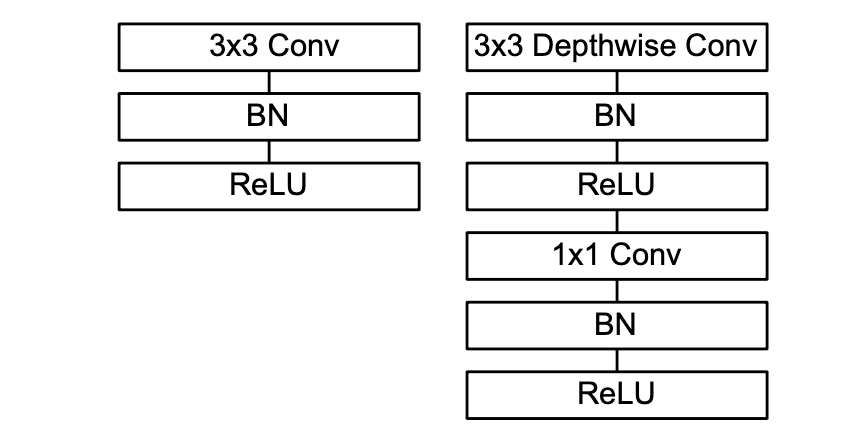
\includegraphics{../pics/COMP.png}

Figure 1: A comparison between standardard convolution layer (left) and
a depth-wise convolution layer (right)

    MobileNet performs picture feature extraction using a combination of
deep-wise convolutional layers and normal convolutional layers.
MobileNet with depth-wise separable convoutional layers performs
somewhat worse than Conv MobileNet (MobileNet built with full
convolutions) (71.7 percent and 70.6 percent on ImageNet). However, the
latter has a far fewer number of parameters (29.3 millions versus 4.2
millions). A smaller number of model parameters is a significant
advantage in reducing model size and inference time, which is very
suitable to be deployed on mobile devices.

    \hypertarget{experiment-process}{%
\subsection{Experiment Process}\label{experiment-process}}

This project consists of three files: load data.py, main.py, and VGG.py.
The first method is for reading raw picture data into tensor. When it
comes to training data, the RandomHorizontalFlip technique is utilized
to horizontally flip training images. With the use of parameter
traindata\_size and valdata\_size, load data.py separates training and
validation data and makes the size controllable . Special methods are
used in the design of load data.py to make the class method more
efficient. The parameter setting function, as well as the training and
validation programs, are all included in main.py. To acquire the
performance of the present model parameters, a validation set is
implemented immediately after training. The model is saved as model.pt
once each epoch is completed. VGG.py contains the neural network models
VGG16 and VGG19, which I created by myself.

    \hypertarget{parameters-comparison}{%
\subsubsection{Parameters comparison}\label{parameters-comparison}}

This section reports experiment result. There are six experiments in
total: epoch number, learning rate, batch size, optimizer and training
data size. In each of them, one parameter is modified. The first
experiment group is the standard group, which can be regarded as the
baseline.

    \hypertarget{standard-group}{%
\paragraph{Standard Group}\label{standard-group}}

This experiment group set epoch number as \textbf{50}, learning rate as
\textbf{0.0001}, batch size as \textbf{16} and dataset parameters as
\textbf{0.6 and 0.95}. The training process is shown in figure2 and
figure 3 as follows:

    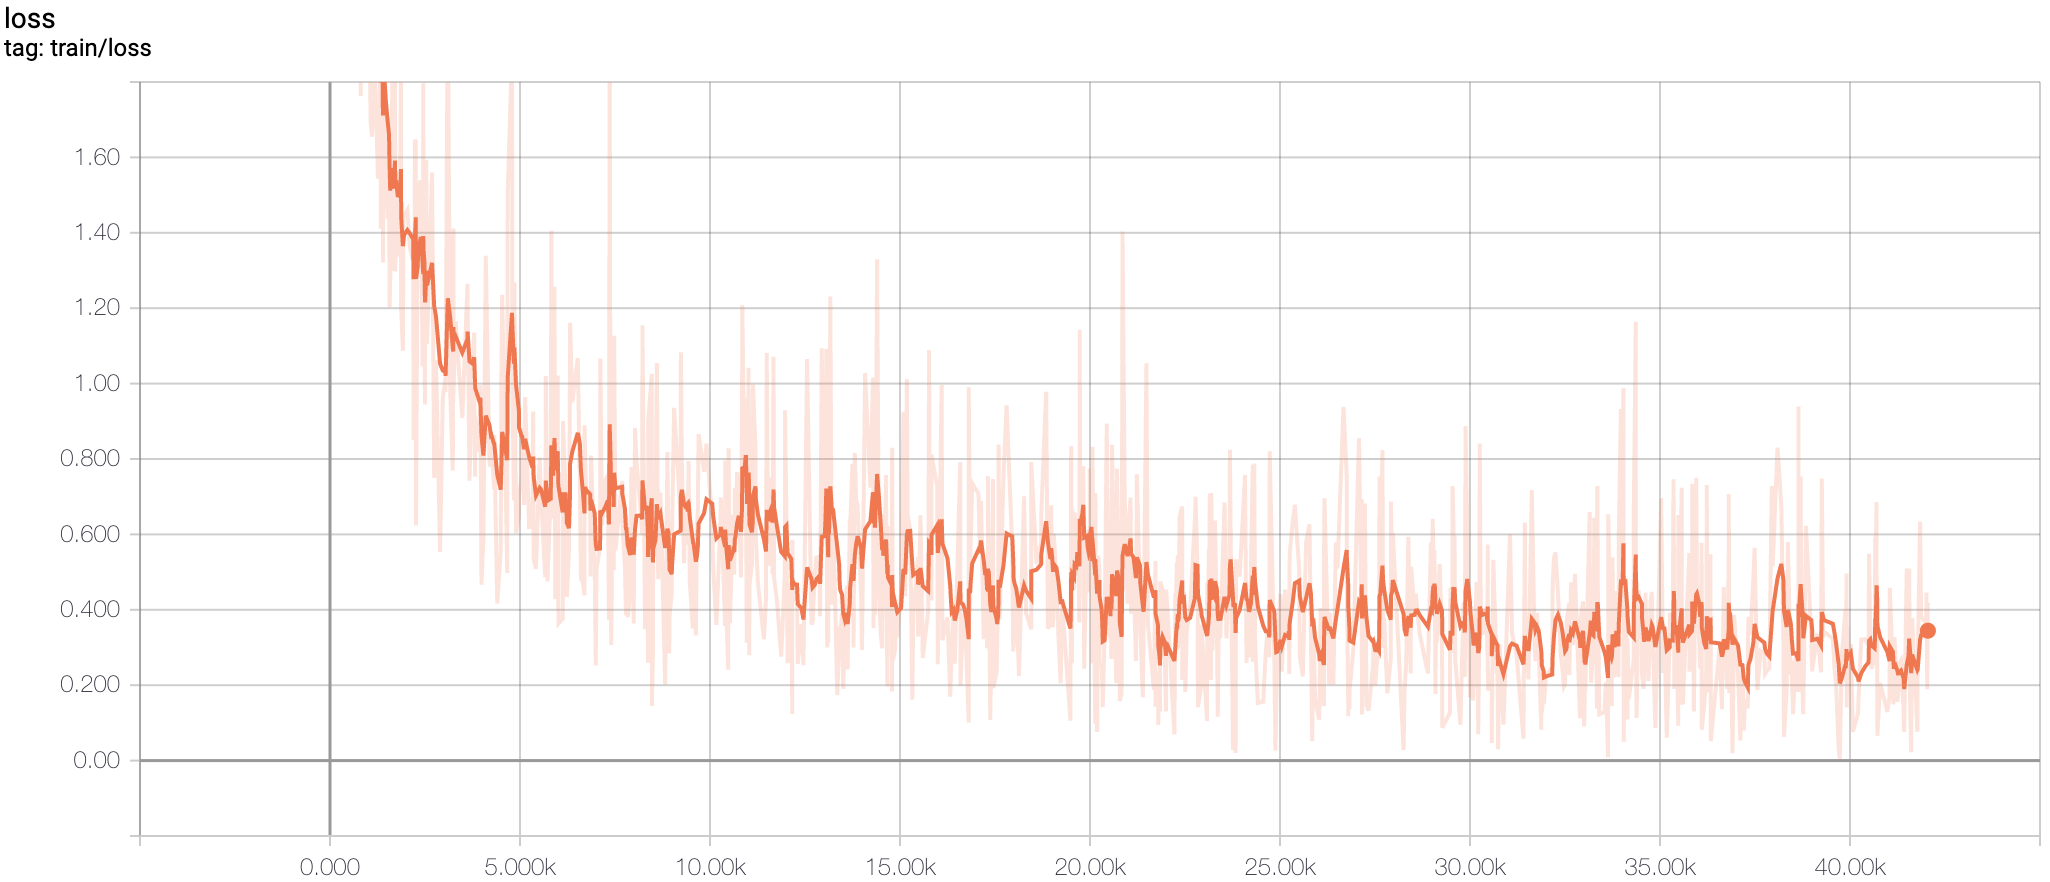
\includegraphics{../pics/SG_1.png}

Figure 2: Loss curve while training in standard group

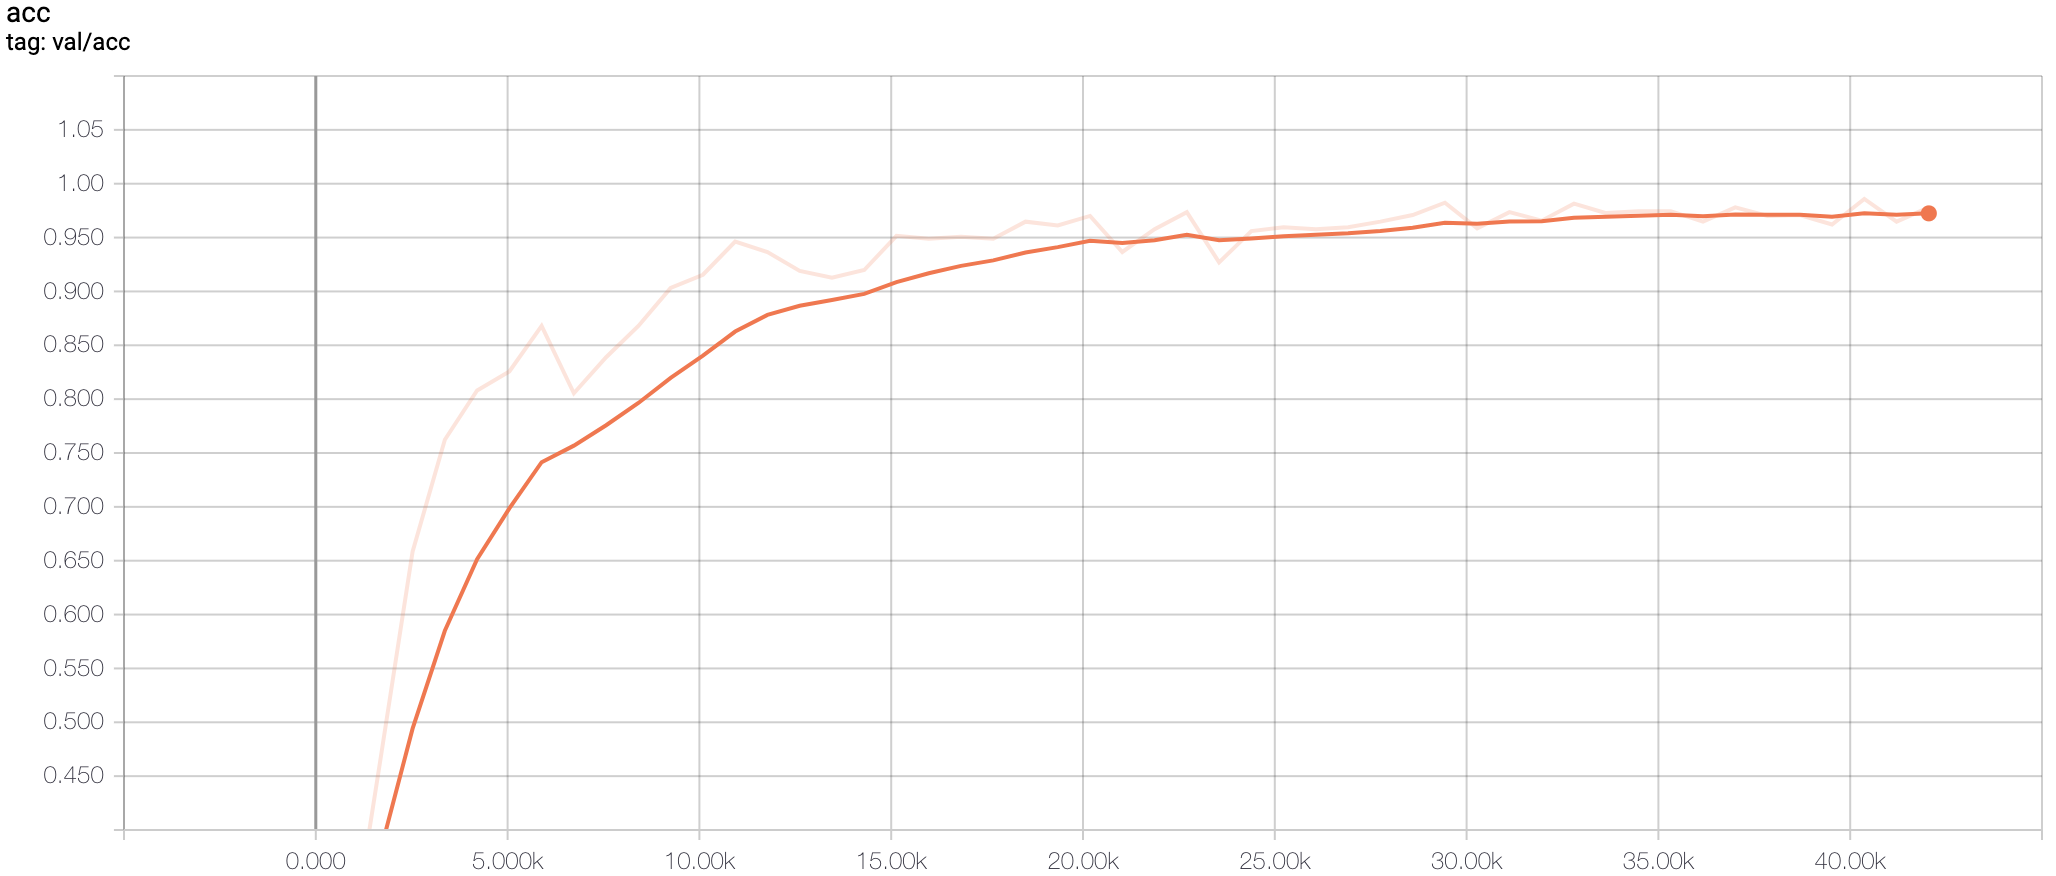
\includegraphics{../pics/SG_2.png}

Figure 3: Accuracy curve while training in standard group

    The loss value starts to drop from the beginning of training and
stabilizes at the global step of 25k, as shown in the graphs above.
After a while, accuracy hits around 0.97, and loss drops to
approximately 0.2 to 0.4.

    \hypertarget{different-epoch-number}{%
\paragraph{Different Epoch number}\label{different-epoch-number}}

This experiment group set epoch number as \textbf{25}, learning rate as
\textbf{0.0001}, batch size as \textbf{16} and dataset parameters as
\textbf{0.6 and 0.95}. The following figures, figure 4 and figure 5,
show the training process:

    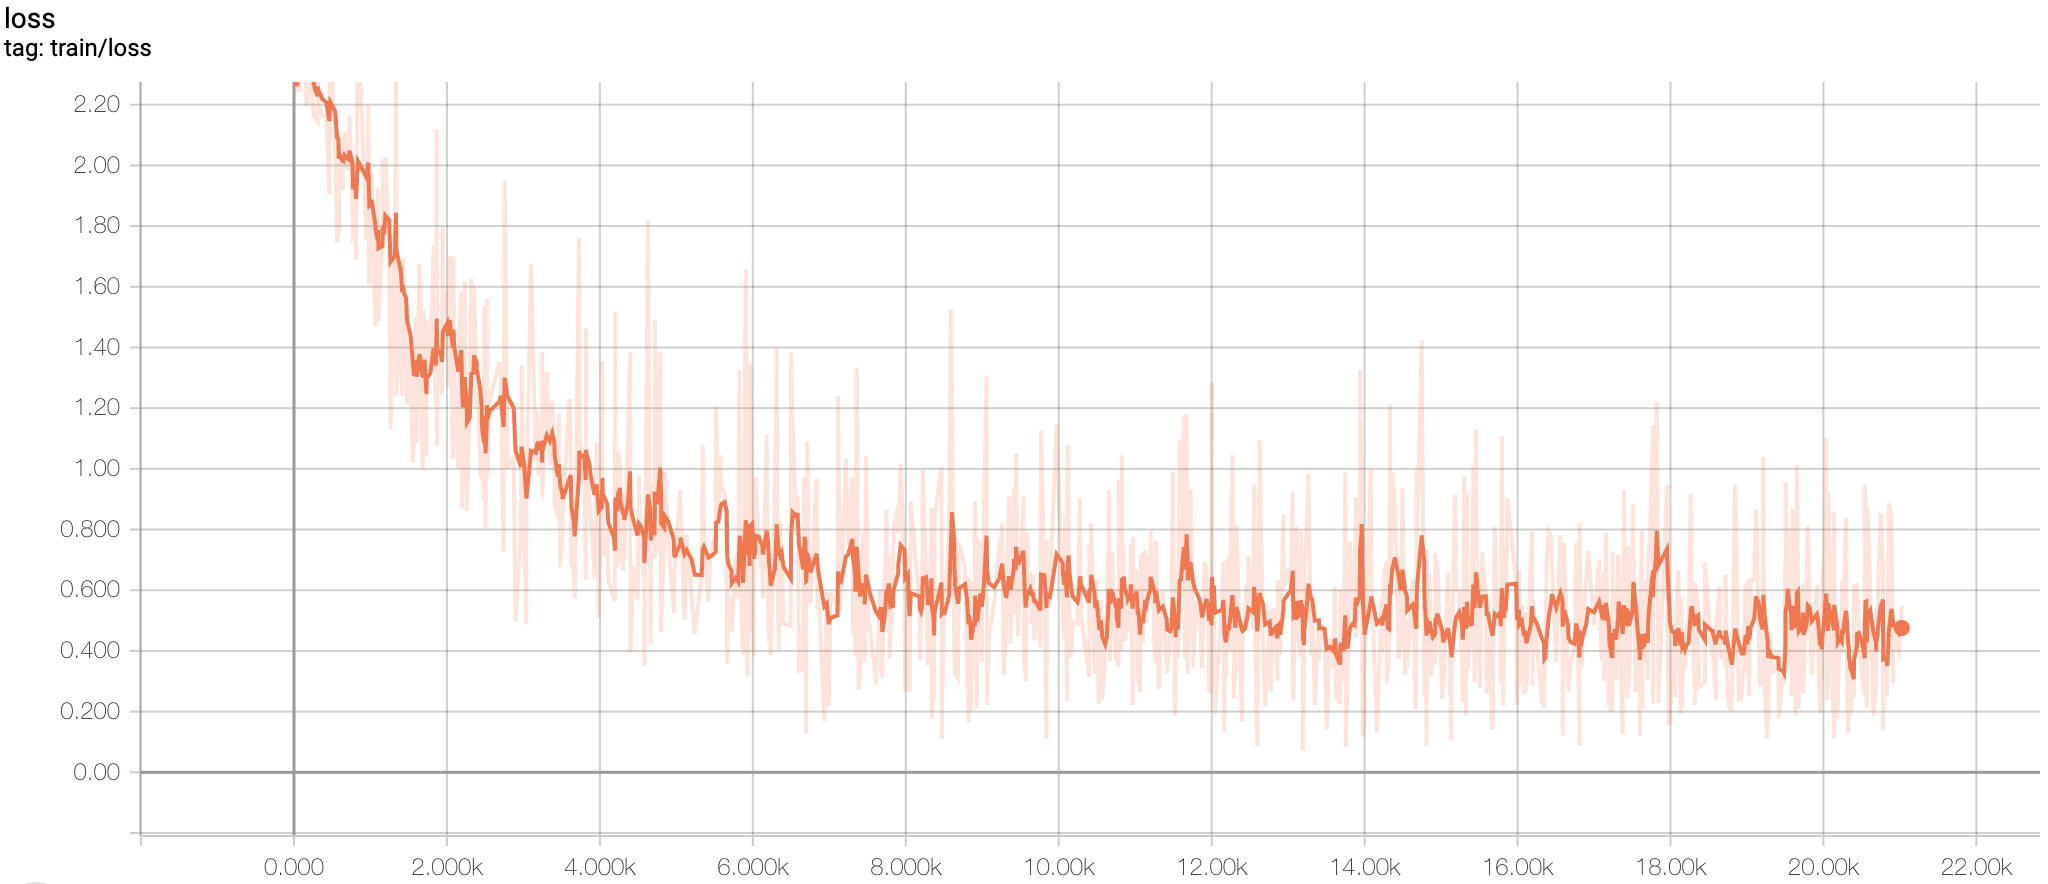
\includegraphics{../pics/Epoch_1.png}

Figure 4: Loss curve while training in small epoch number group

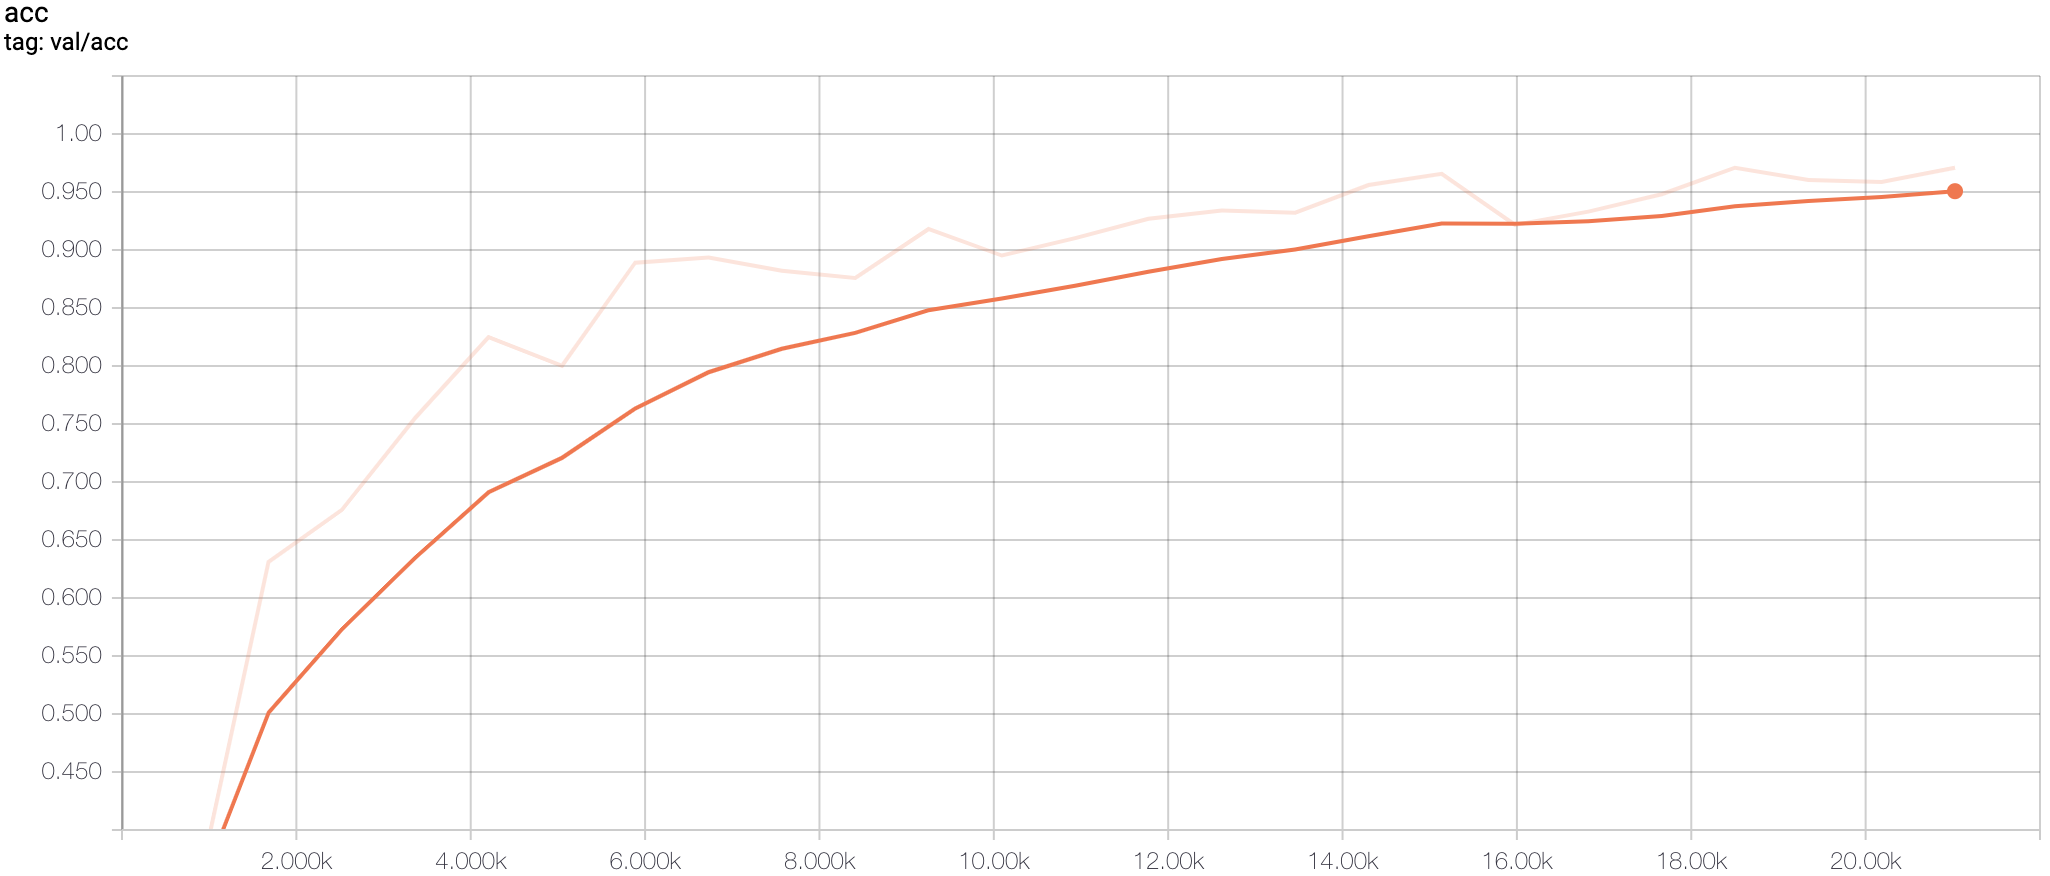
\includegraphics{../pics/Epoch_2.png}

Figure 5: Loss curve while training in small epoch number group

    In comparison to the standard group, the preceding figures show that,
while the loss value is nearly stable, accuracy is not. In the end, it
hovers around 0.95, which is somewhat lower than the typical group's
accuracy rate. Finally, sufficient training epoches are required to
ensure that the neural network is properly trained and that its best
performance is demonstrated.

    \hypertarget{different-learning-rate}{%
\paragraph{Different Learning Rate}\label{different-learning-rate}}

This experiment group set epoch number as \textbf{50}, learning rate as
\textbf{0.001}, batch size as \textbf{16} and dataset parameters as
\textbf{0.6 and 0.95}. Figure 6 and figure 7 show the training process:

    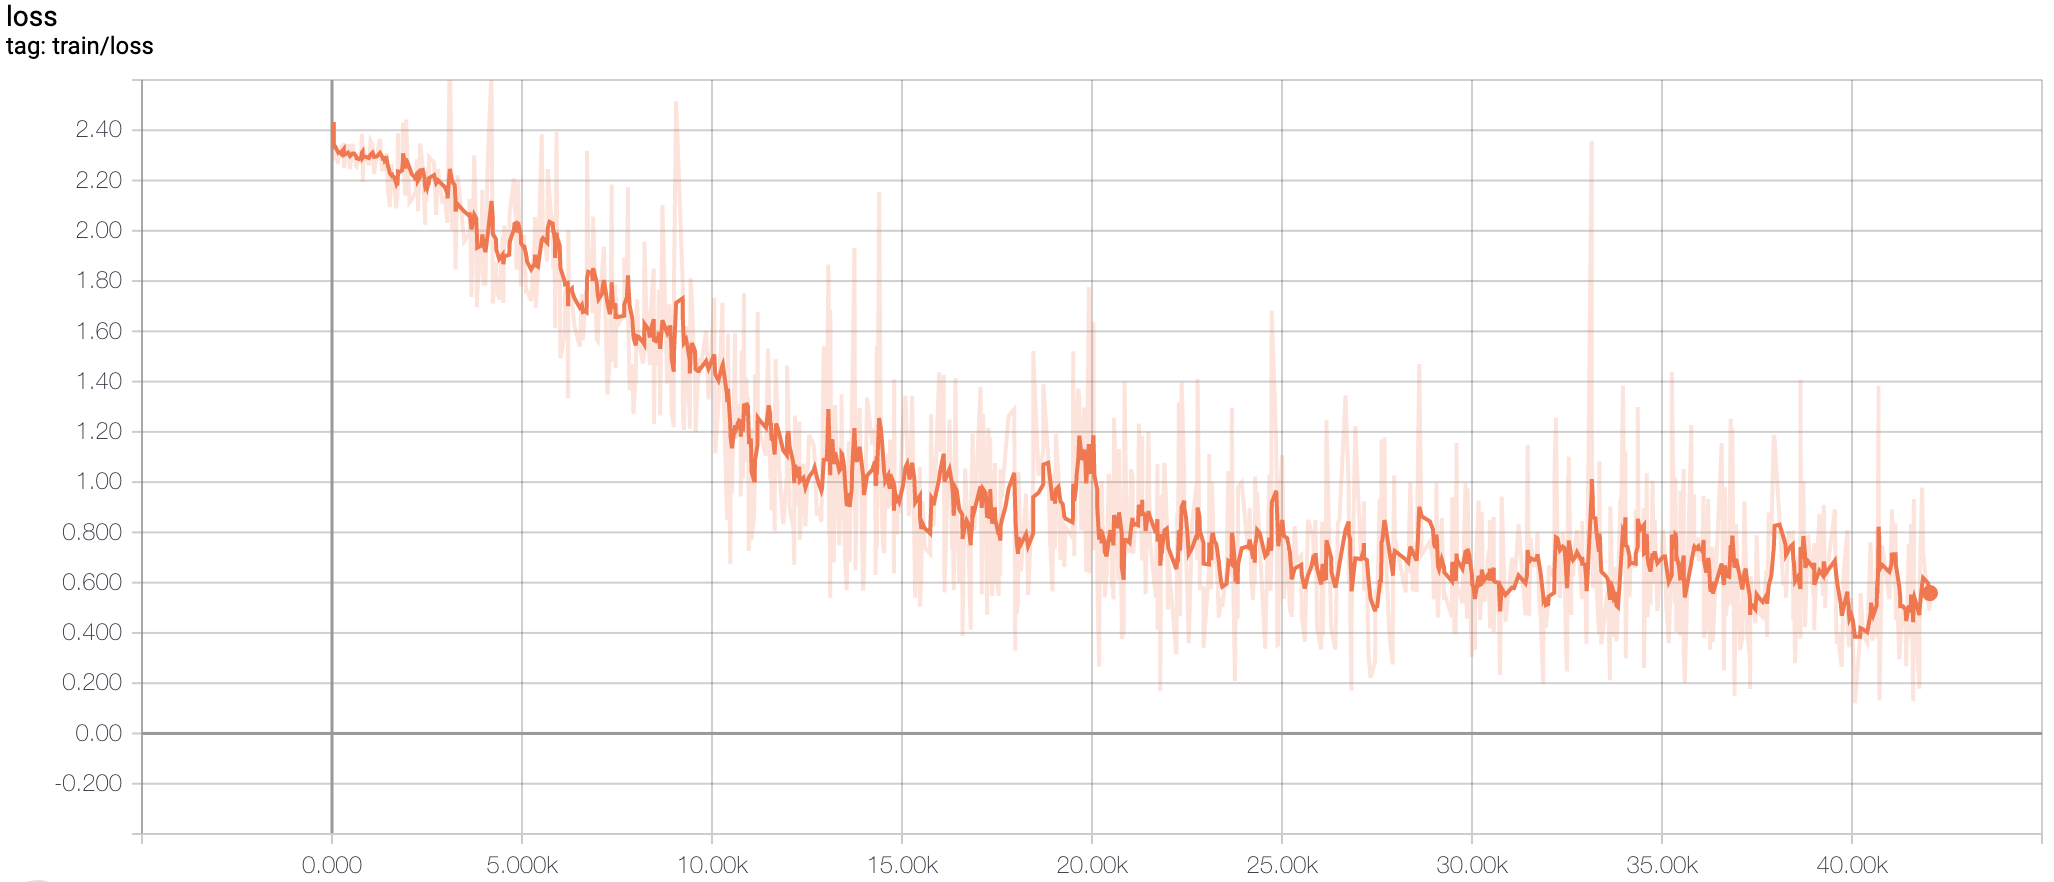
\includegraphics{../pics/LR_1.png}

Figure 6: Loss curve while training in large learning rate group

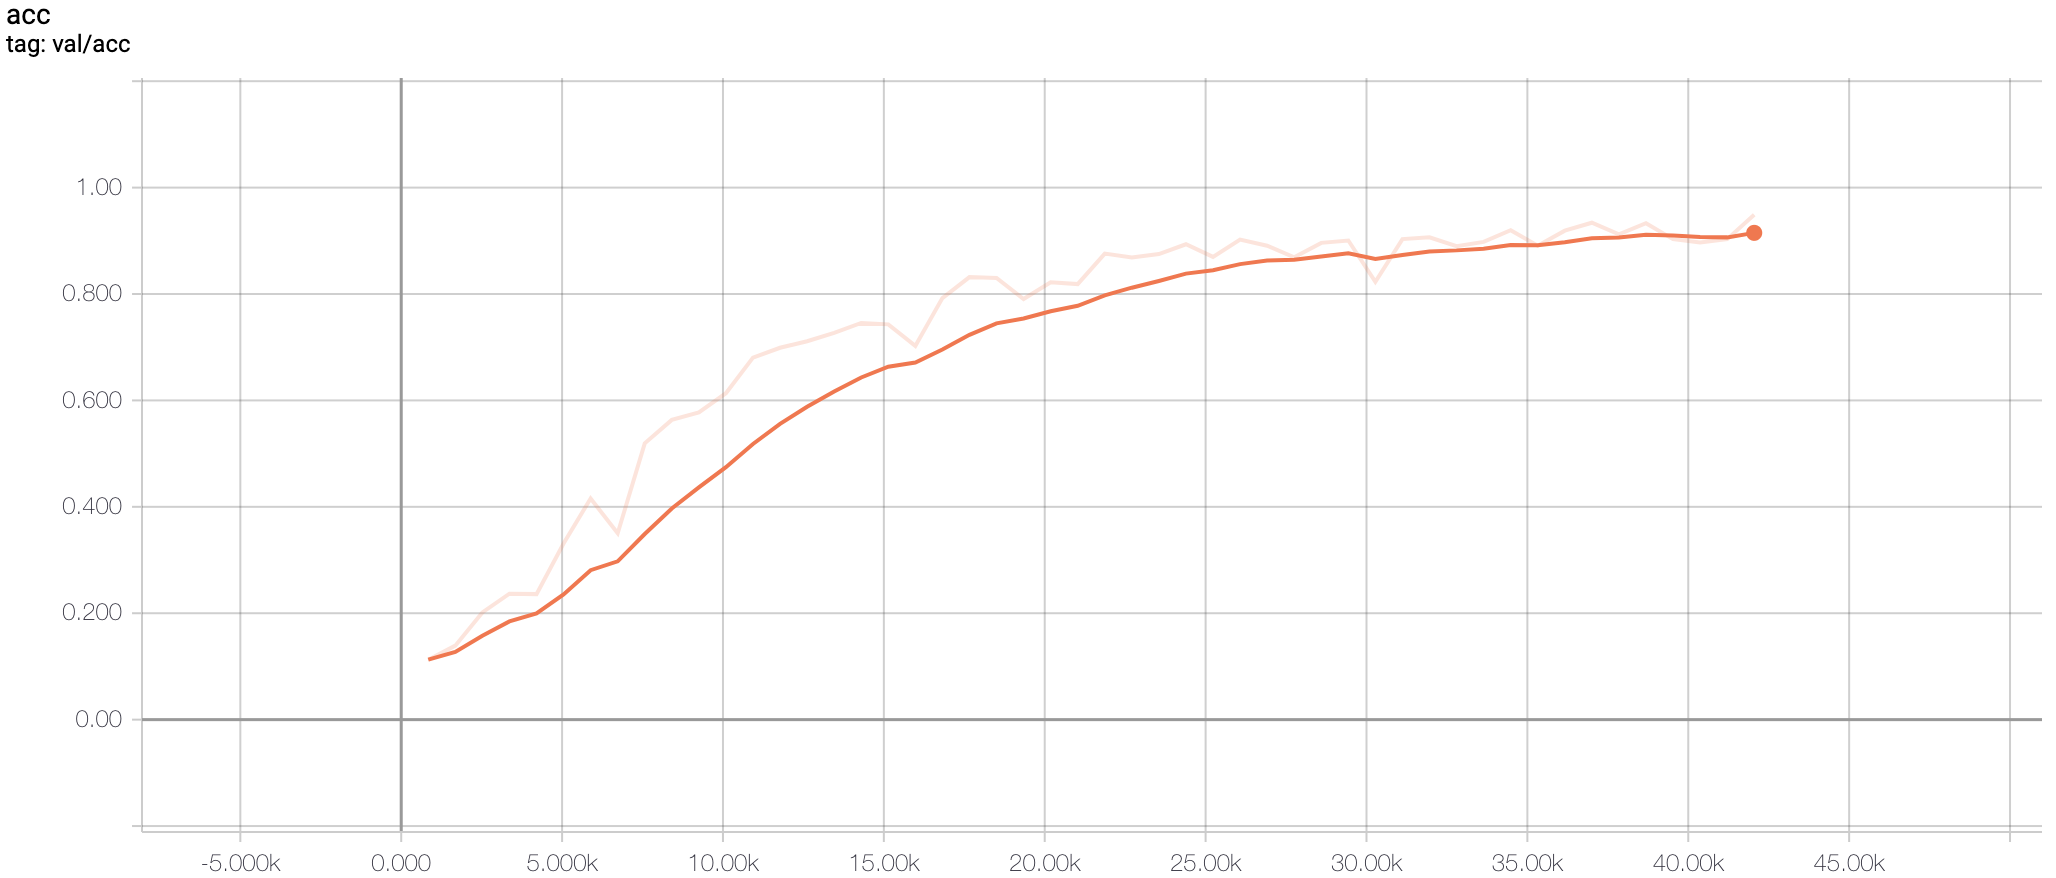
\includegraphics{../pics/LR_2.png}

Figure 7: Loss curve while training in large learning rate group

    The learning rate is changed from 0.0001 to 0.001 in this experiment.
When it comes to the loss graph, it's worth noting that the loss curve
sways a lot during training. It fluctuates between 0.4 and 0.8 after 50
epoches of training, compared to 0.4 to 0.6 in the control group. This
experiment group's accuracy (about 95\%) is also lower than the standard
group's (around 96 percent). Finally, it is important to note that the 
learning rate for training deep neural networks is usually set as 0.0001 
or 0.00001, which is an empiric value.

    \hypertarget{different-batch-size}{%
\paragraph{Different Batch Size}\label{different-batch-size}}

This experiment group set epoch number as \textbf{50}, learning rate as
\textbf{0.0001}, batch size as \textbf{8} and dataset parameters as
\textbf{0.6 and 0.95}. Figure 8 and figure 9 show the training process:

    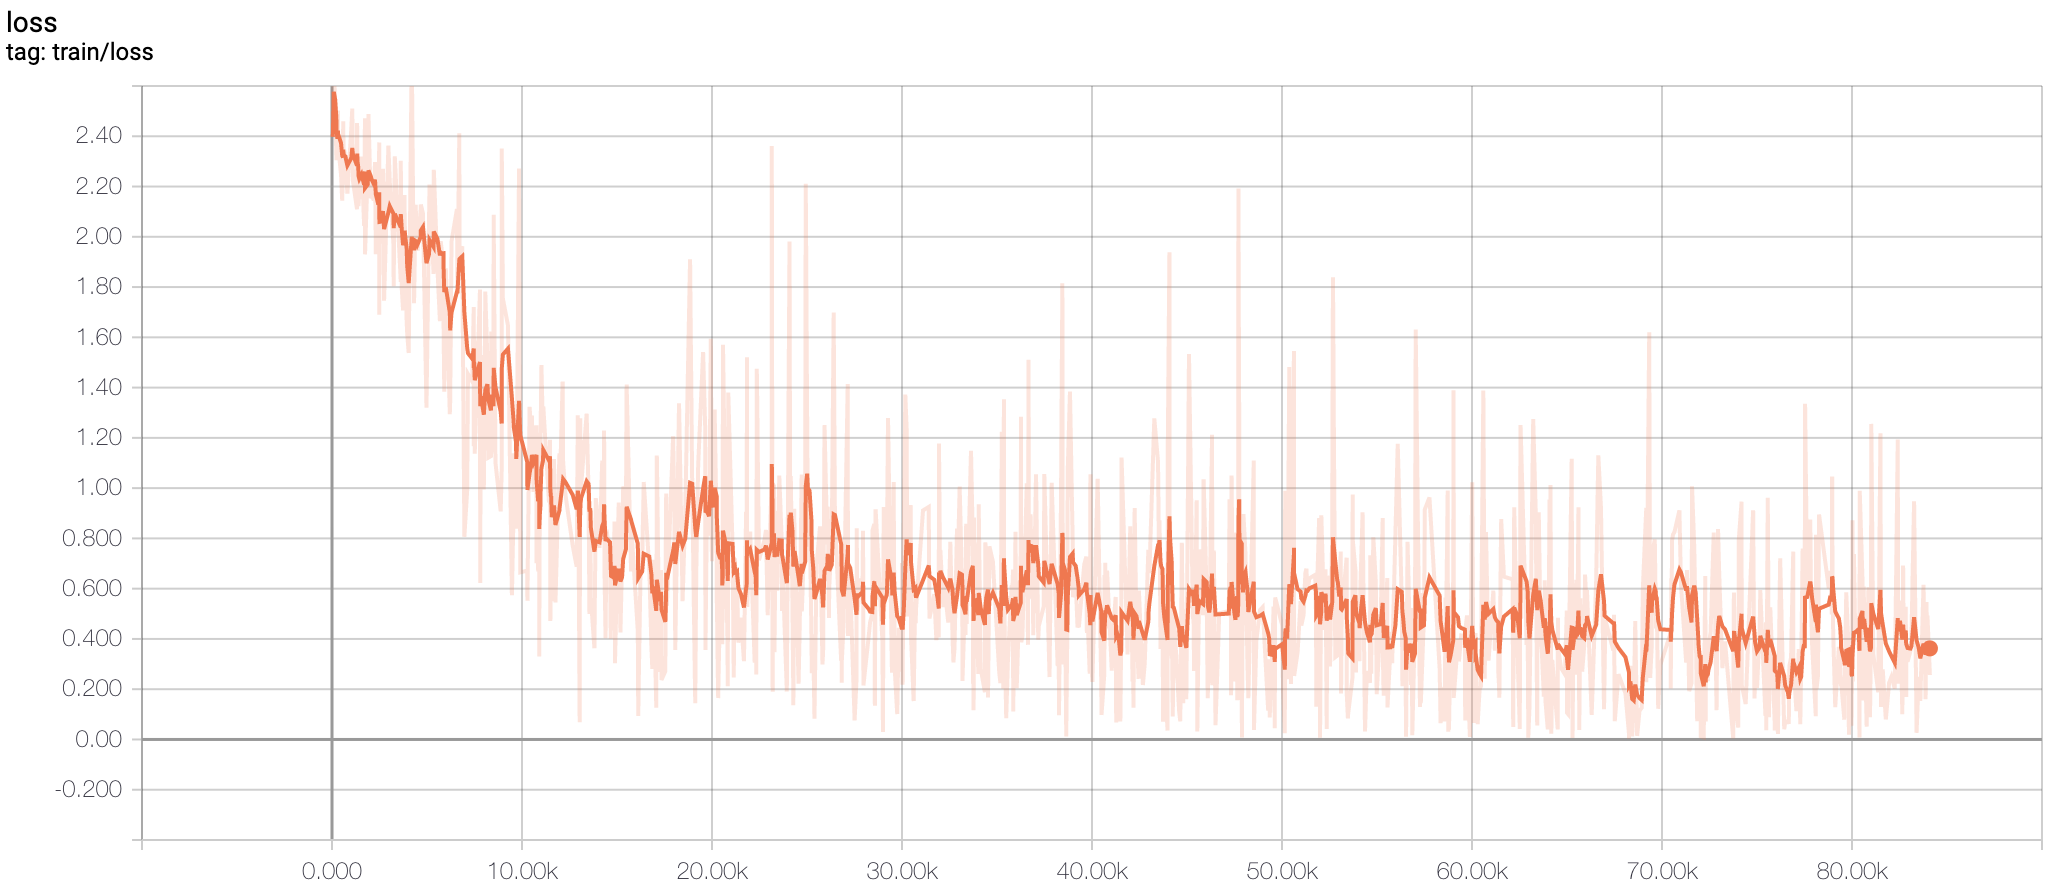
\includegraphics{../pics/BS_1.png}

Figure 8: Loss curve while training in small batch size group

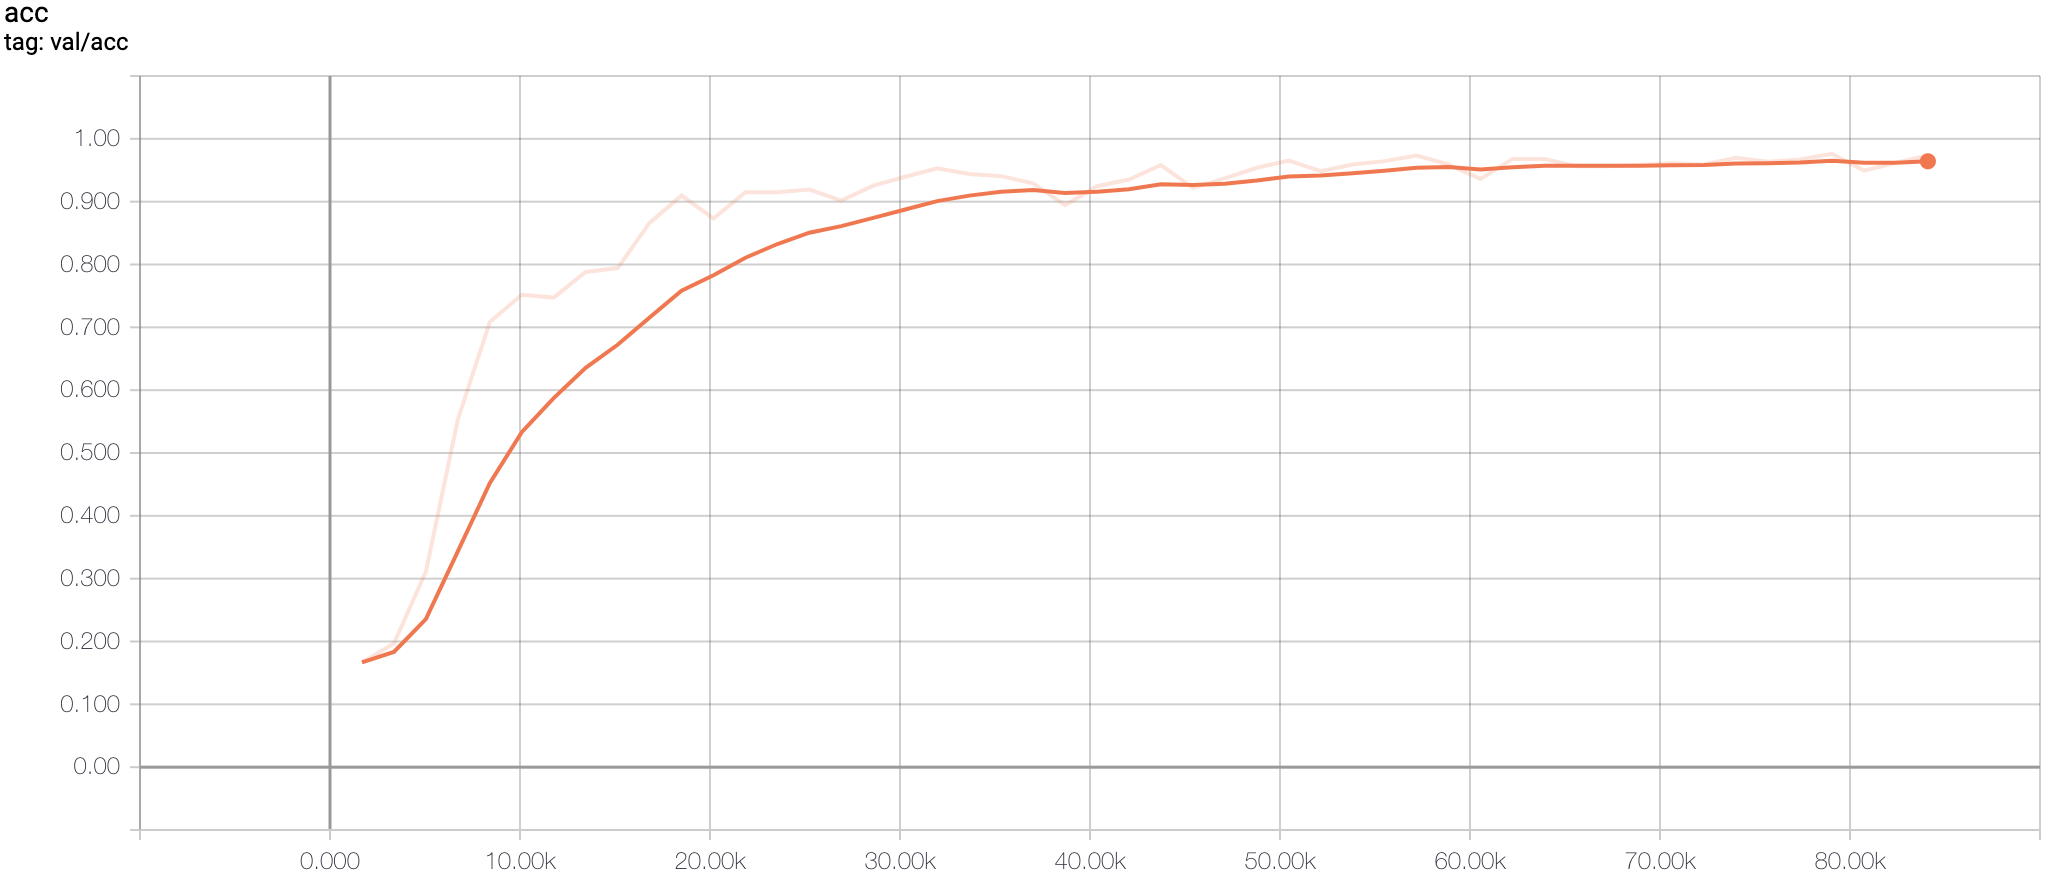
\includegraphics{../pics/BS_2.png}

Figure 9: Loss curve while training in small batch size group

    Batch size is set to 8 instead of 16 in this experiment group. As a
result, the worldwide step count has risen to 100,000. Meanwhile, it's
worth noting that the training period will be longer and the loss curve
appears to oscillate more than the standard group's.

    \hypertarget{sgd-over-adam}{%
\paragraph{SGD over Adam}\label{sgd-over-adam}}

This experiment group set epoch number as \textbf{50}, learning rate as
\textbf{0.0001}, batch size as \textbf{16} and dataset parameters as
\textbf{0.6 and 0.95}. However, the optimizer uses SGD rather than
Adam{[}8{]}. Figure 10 and figure 11 show the training process:

    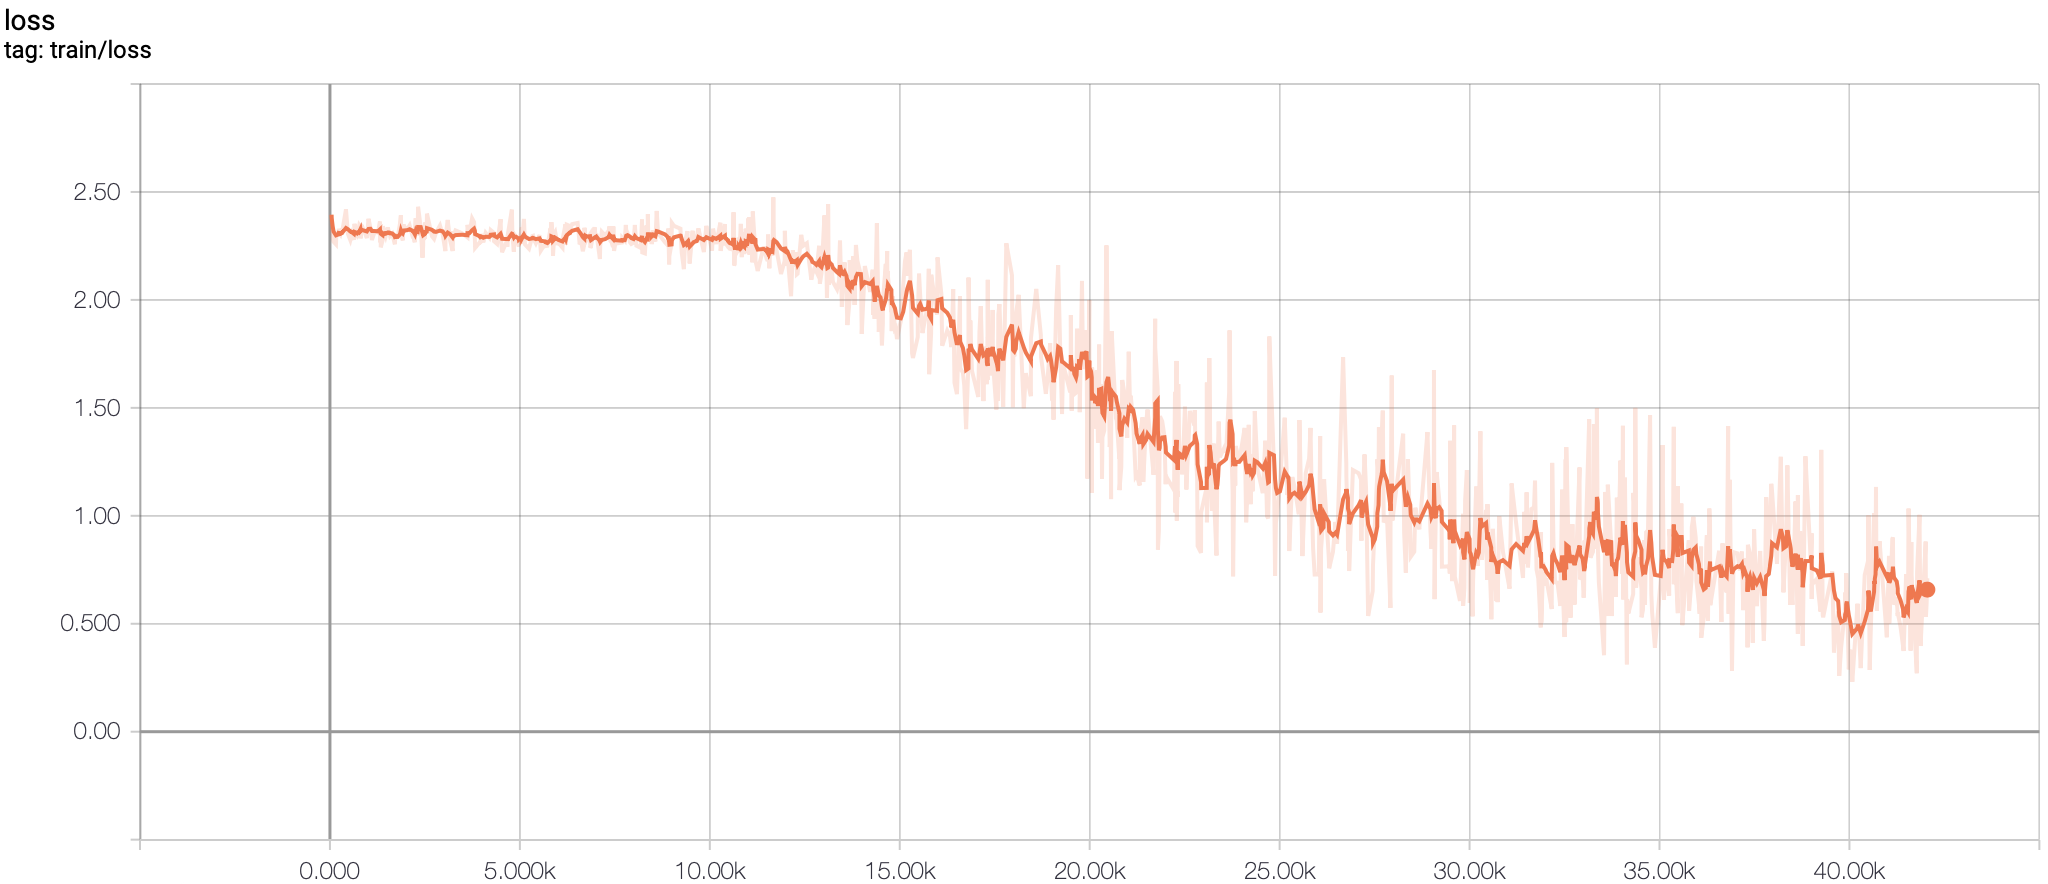
\includegraphics{../pics/SGD_1.png}

Figure 10: Loss curve while training in SGD optimizer group

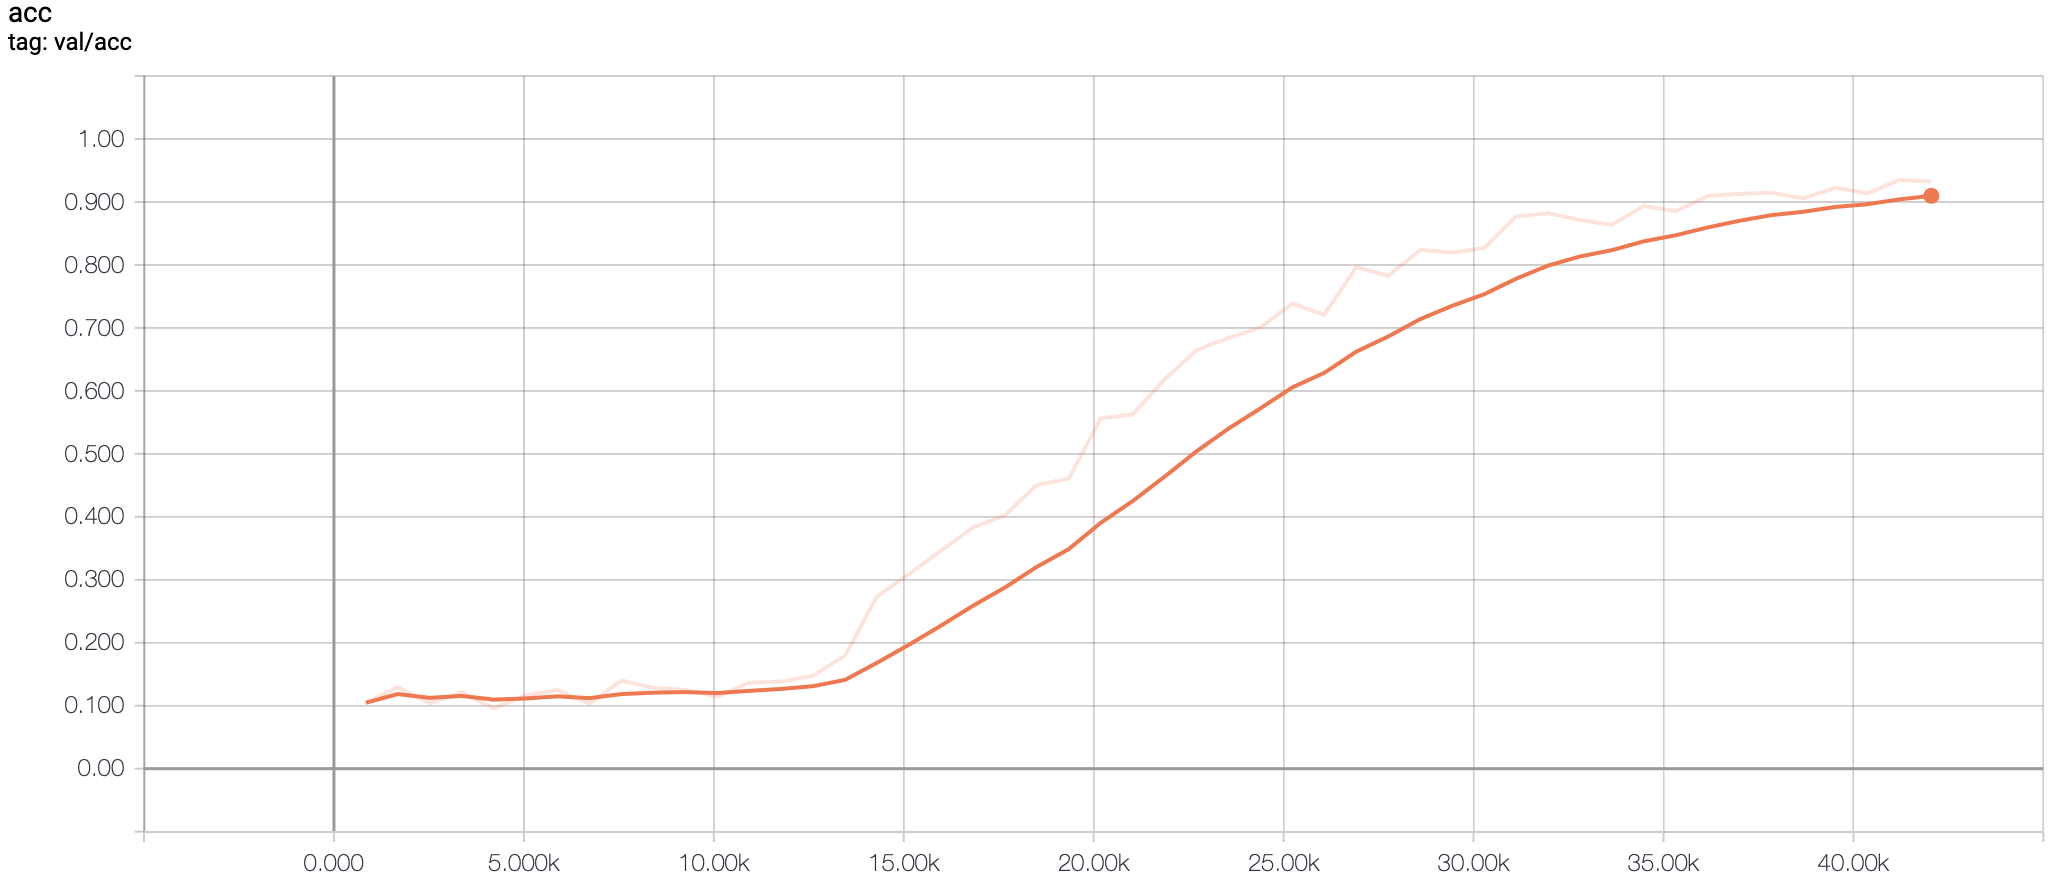
\includegraphics{../pics/SGD_2.png}

Figure 11: Loss curve while training in SGD optimizer group

    This study group compares the effects of several optimizers on the
training process. When compared to the Adam optimizer, the loss in SGD
decays far more slowly. It only starts to decay at a global step of
roughly 10k, owing to the fact that the SGD optimizer is more likely to
fall into a local minimum. The accuracy curve follows a similar pattern.
After the 13th global step, it only starts to increase. The accuracy
eventually arrives at 90\%, which is lower than the standard group. Adam
is a superior Optimizer than SGD, according to the trial.

    \hypertarget{different-training-size}{%
\paragraph{Different Training Size}\label{different-training-size}}

This experiment group set epoch number as \textbf{50}, learning rate as
\textbf{0.0001}, batch size as \textbf{16} and dataset parameters as
\textbf{0.6 and 0.95}. The training process is shown in figure 12 and
figure 13:

    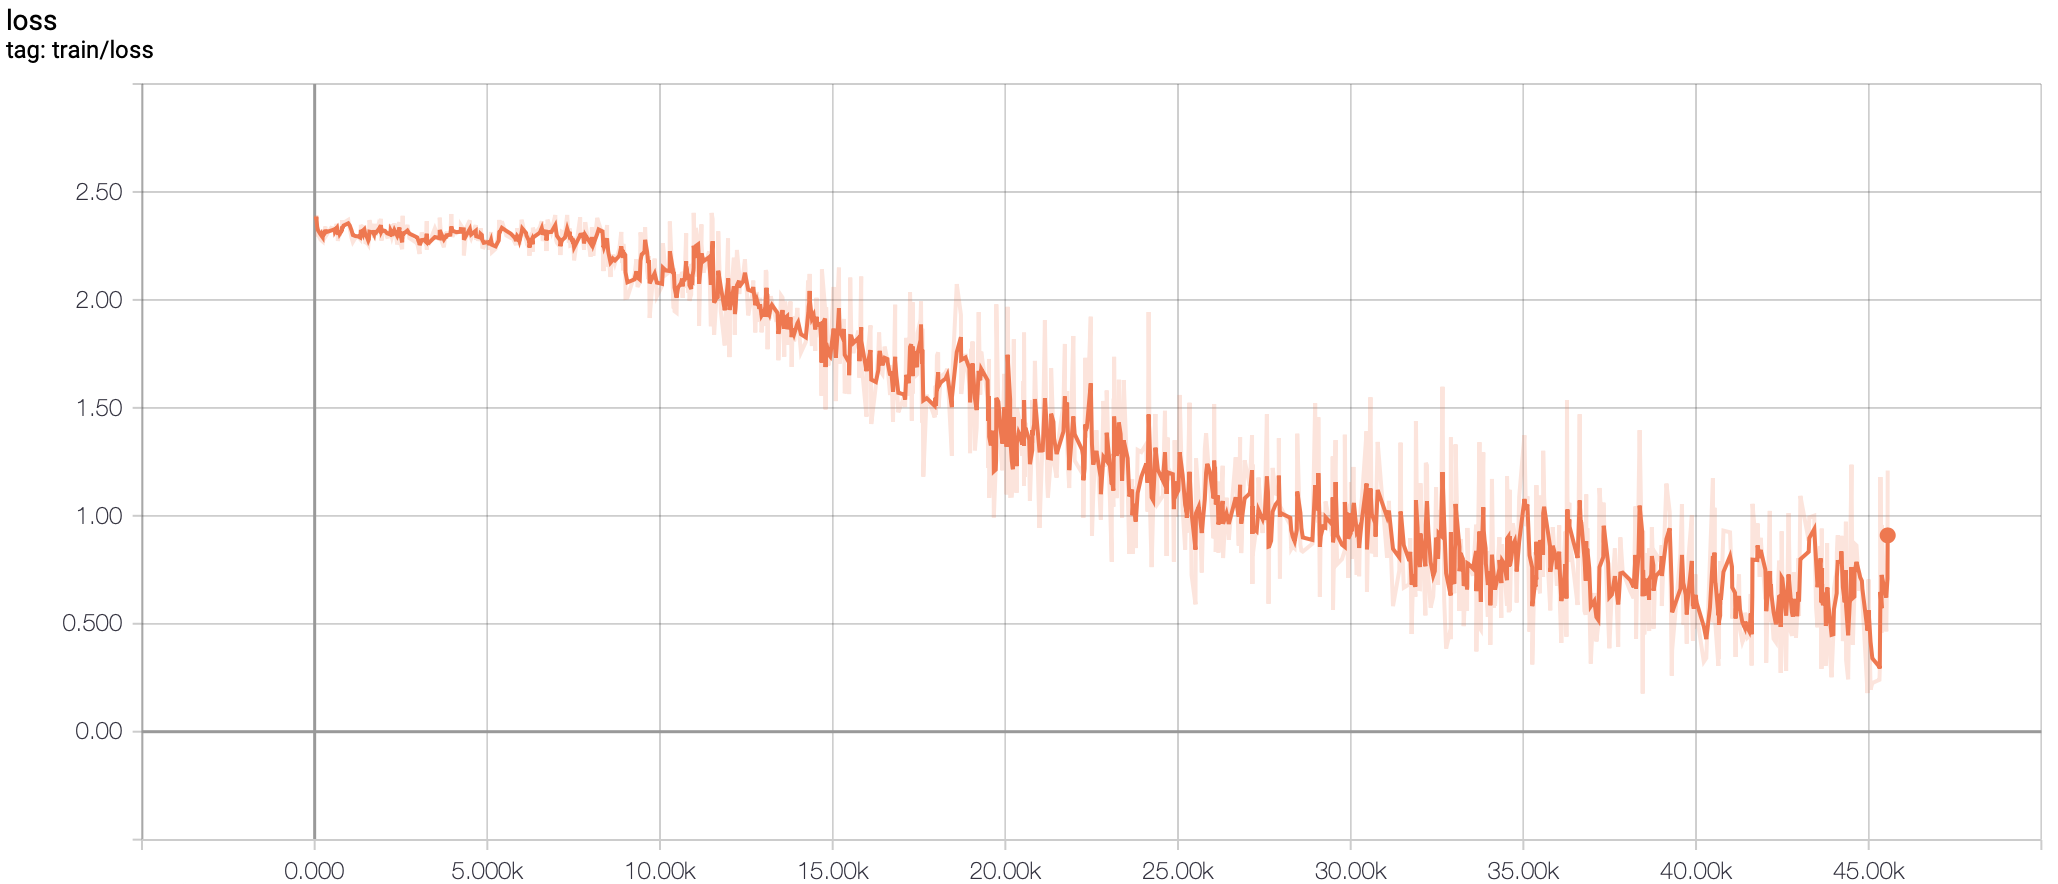
\includegraphics{../pics/TS_loss.png}

Figure 12: Loss curve while training in small training data size group

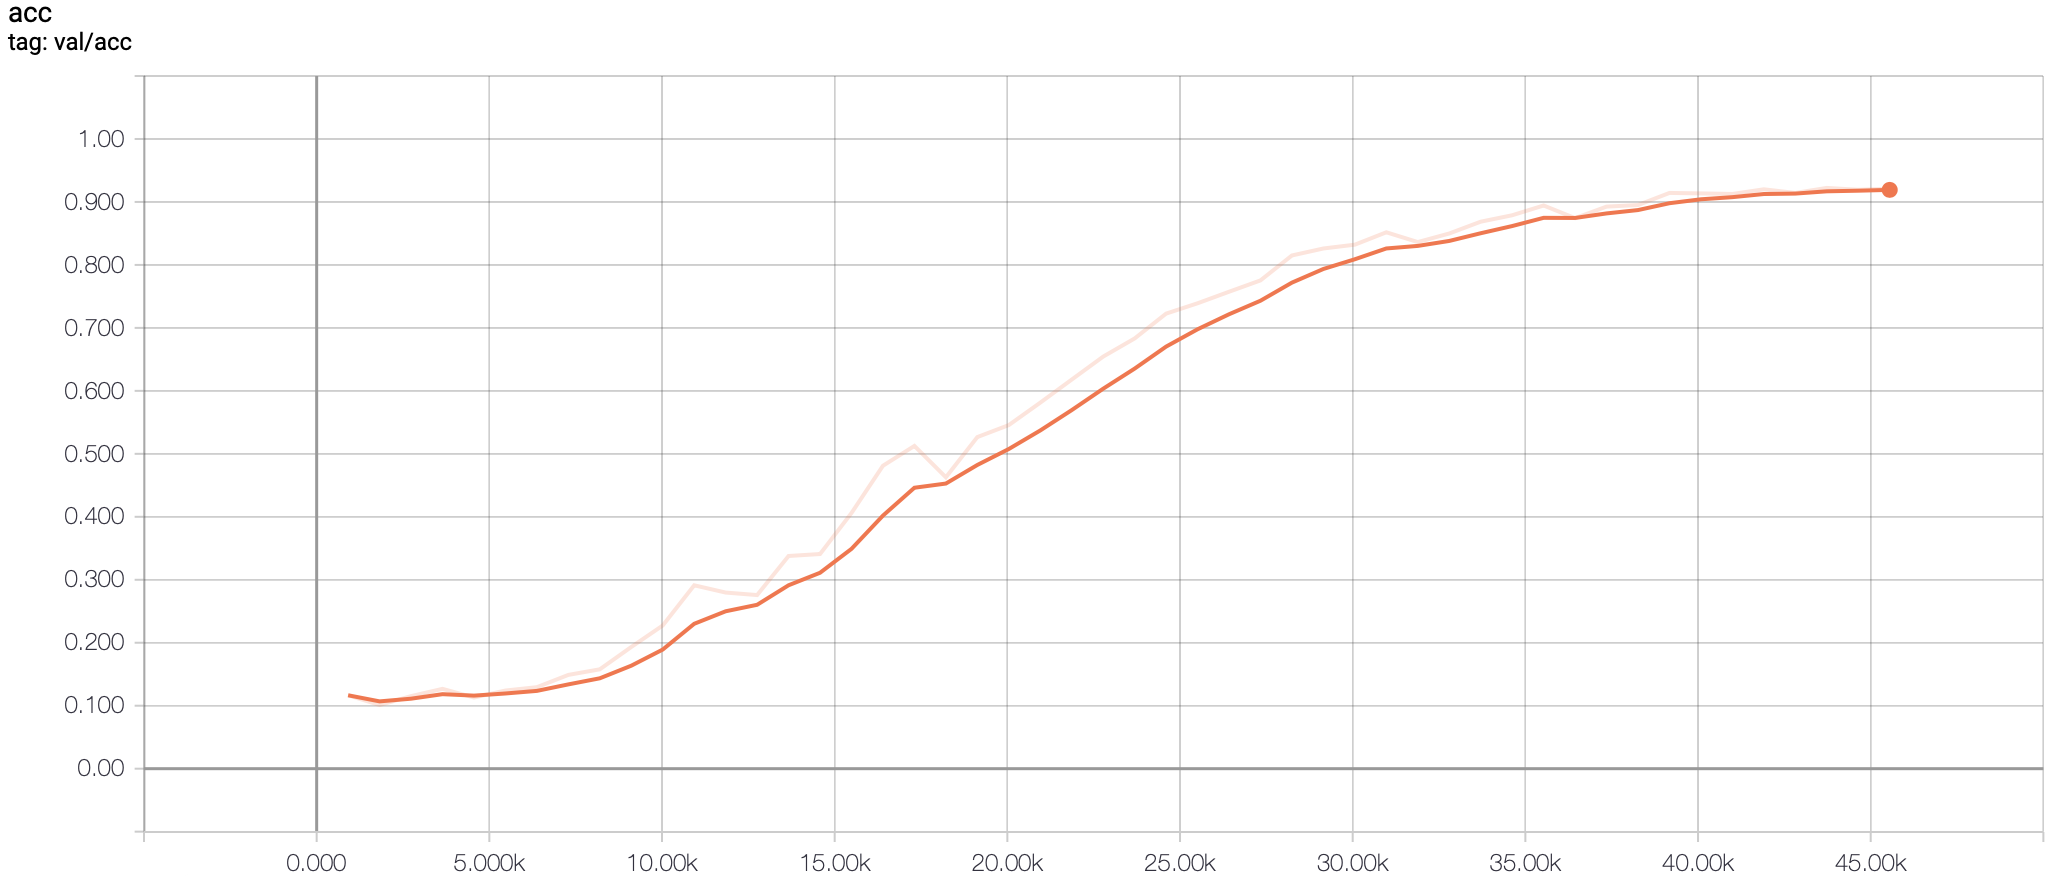
\includegraphics{../pics/TS_ACC.png}

Figure 13: Loss curve while training in small training data size group

    The training data amount is increased in this trial group, and the index
value is raised from 0.6 to 0.65. Meanwhile, the size of the validation
data has been reduced from 0.95 to 0.9. The loss value after training
(between 0.5 to 1) is much bigger than the standard group, as shown in
the graphs above. Finally, the accuracy rate reaches around 91 percent.
The conclusion is intriguing: as the size of the training dataset grows,
the training loss and validation accuracy decrease for the same number
of training epochs. Meanwhile, training the neural network with a larger
dataset necessitates a higher number of training epoch sizes.

    \hypertarget{summary}{%
\subsection{Summary}\label{summary}}

The chart above shows how different hyperparameters affect the training
process. Overall, epoch refers to the overall number of training
iterations, and having a sufficient number of training iterations is
crucial for excellent training accuracy. Because the learning rate
determines how quickly the gradient lowers, a low learning rate usually
results in a slower training process, whereas a high learning rate
produces a lot of oscillation as the loss decreases. When it comes to
batch size, a lower batch size lengthens the training process overall,
but the end accuracy remains the same. The choice of optimizer,
according to the preceding trials, is also crucial in achieving good
training accuracy. Adam outperforms SGD significantly. The Adam
technique can help the training process get to the fitting state faster
and cross the local minimum value more effectively.

Table 2-1 and Table 2-2 reports the accuracy rate and loss rate of all experiments.

\begin{tabular}{|c|c|c|c|c|c|c|}%
\hline
Group & standard group & Different Epoch Number & Learning Rate \\
\hline
Accuracy & 0.97 & 0.95 & 0.92 \\
Loss & 0.2-0.4 & 0.4-0.6 & 0.4-0.8 \\
\hline
\end{tabular}

Table 2-1 Experiment Summary of standard group, epoch number group and learning rate group

\begin{tabular}{|c|c|c|c|c|c|c|}%
    \hline
    Group & Batch Size & SGD & Training data size \\
    \hline
    Accuracy & 0.96 & 0.91 & 0.92 \\
    Loss & 0.2-0.6 & 0.5-1 & 0.5-1 \\
    \hline
    \end{tabular}
    
    Table 2-2 Experiment Summary of batch size group, optimizer group and training data group 

    \hypertarget{conclusion-and-discussion}{%
\section{Conclusion and Discussion}\label{conclusion-and-discussion}}

This project uses MobileNet to classify driver images. Meanwhile, it
investigates how hyperparameter settings affect the training process.
According to the previous analysis, all five parameters have a direct
influence on the training process, with the exception of batch size,
which only influences the overall global step size and then the total
training duration.

Despite the foregoing findings, a deeper investigation into parameter
tweaking is still required. Despite the fact that a lower learning rate
means a lower oscillation, a low learning rate slows down the training
process. The employment of a dynamic learning rate is a frequent
solution to this problem. This approach starts with a high learning
rate, but it gradually decreases after each epoch. Both the training
time and the oscillation issue are balanced as a result. The batch size
is in a similar scenario. If the training is done on GPU, a large batch
size necessitates a large graphic memory, and if the dataset is too
huge, it may become a problem. Another element that must be carefully
studied is the epoch number. The neural network model may not be fully
trained if the epoch number is too small. However, if it becomes too
large, the additional training time will become unnecessary. Finally,
selecting an optimizer is critical. As can be seen in the prior
analysis, Adam is a newer and superior optimizer than SGD.

In the future, a more detailed comparison should be considered. For
example, a test of whether the aforementioned dynamic learning rate
method improves the overall training process in the sense of accuracy
and training duration. In addition, a smarter way of training the neural
network can be used. For example, as proposed in Vision
Transformer{[}5{]}, comparing the results of the current training round
with the results of the verification set regularly until the accuracy
does not improve beyond a given range is a superior training strategy.
This strategy is smarter and better than giving a fixed number of
training epcoh.

    \hypertarget{reference}{%
\section{Reference}\label{reference}}

{[}1{]} LeCun, Y., Boser, B., Denker, J.S., Henderson, D., Howard, R.E.,
Hubbard, W. and Jackel, L.D., 1989. Backpropagation applied to
handwritten zip code recognition. Neural computation, 1(4), pp.541-551.

{[}2{]} Simonyan, K. and Zisserman, A., 2014. Very deep convolutional
networks for large-scale image recognition. arXiv preprint
arXiv:1409.1556.

{[}3{]} He, K., Zhang, X., Ren, S. and Sun, J., 2016. Deep residual
learning for image recognition. In Proceedings of the IEEE conference on
computer vision and pattern recognition (pp.~770-778).

{[}4{]} Szegedy, C., Liu, W., Jia, Y., Sermanet, P., Reed, S., Anguelov,
D., Erhan, D., Vanhoucke, V. and Rabinovich, A., 2015. Going deeper with
convolutions. In Proceedings of the IEEE conference on computer vision
and pattern recognition (pp.~1-9).

{[}5{]} Wang, J., Sun, K., Cheng, T., Jiang, B., Deng, C., Zhao, Y.,
Liu, D., Mu, Y., Tan, M., Wang, X. and Liu, W., 2020. Deep
high-resolution representation learning for visual recognition. IEEE
transactions on pattern analysis and machine intelligence.

{[}6{]} Howard, A.G., Zhu, M., Chen, B., Kalenichenko, D., Wang, W.,
Weyand, T., Andreetto, M. and Adam, H., 2017. Mobilenets: Efficient
convolutional neural networks for mobile vision applications. arXiv
preprint arXiv:1704.04861.

{[}7{]} Dosovitskiy, A., Beyer, L., Kolesnikov, A., Weissenborn, D.,
Zhai, X., Unterthiner, T., Dehghani, M., Minderer, M., Heigold, G.,
Gelly, S. and Uszkoreit, J., 2020. An image is worth 16x16 words:
Transformers for image recognition at scale. arXiv preprint
arXiv:2010.11929.

{[}8{]} Kingma, D.P. and Ba, J., 2014. Adam: A method for stochastic
optimization. arXiv preprint arXiv:1412.6980.

{[}9{]} Géron, A., 2019. Hands-on machine learning with Scikit-Learn,
Keras, and TensorFlow: Concepts, tools, and techniques to build
intelligent systems. O'Reilly Media.

{[}10{]} Pointer, I., 2019. Programming PyTorch for Deep Learning:
Creating and Deploying Deep Learning Applications. " O'Reilly Media,
Inc.".


    % Add a bibliography block to the postdoc
    
    
    
\end{document}
